%  -----------------------------------------------------------------------------
%  Author         : Bimalka Piyaruwan Thalagala
%  GitHub         : https://github.com/bimalka98
%  Date Created   : 01.09.2020
%  Last Modified  : 13.09.2020
%  -----------------------------------------------------------------------------

\documentclass[a4paper,11pt]{article}%,twocolumn
%% packages

\usepackage{blindtext} % needed for creating dummy text passages
%\usepackage{ngerman} % needed for German default language
\usepackage{amsmath} % needed for command eqref
\usepackage{amssymb} % needed for math fonts
\usepackage[colorlinks=true,breaklinks]{hyperref} % needed for creating hyperlinks in the document, the option colorlinks=true gets rid of the awful boxes, breaklinks breaks lonkg links (list of figures), and ngerman sets everything for german as default hyperlinks language
\usepackage[hyphenbreaks]{breakurl} % ben�tigt f�r das Brechen von URLs in Literaturreferenzen, hyphenbreaks auch bei links, die �ber eine Seite gehen (mit hyphenation).
\usepackage{xcolor}
\definecolor{c1}{rgb}{0,0,1} % blue
\definecolor{c2}{rgb}{0,0.3,0.9} % light blue
\definecolor{c3}{rgb}{0.3,0,0.9} % red blue
\hypersetup{
    linkcolor={c1}, % internal links
    citecolor={c2}, % citations
    urlcolor={c3} % external links/urls
}
%\usepackage{cite} % needed for cite
\usepackage[square,authoryear]{natbib} % needed for cite and abbrvnat bibliography style
\usepackage[nottoc]{tocbibind} % needed for displaying bibliography and other in the table of contents
\usepackage{graphicx} % needed for \includegraphics 
\usepackage{longtable} % needed for long tables over pages
\usepackage{bigstrut} % needed for the command \bigstrut
\usepackage{enumerate} % needed for some options in enumerate
%\usepackage{todonotes} % needed for todos
\usepackage{makeidx} % needed for creating an index
\makeindex
\usepackage{gensymb}
\usepackage{url}
\usepackage{psfrag}
\usepackage{multirow}
\usepackage{subfigure}
%% page settings

\usepackage[top=20mm, bottom=20mm,left=25mm,right=25mm]{geometry} % needed for page border settings
\parindent=0mm % for space of first line of new text block
\sloppy % for writing with hyphenless justification (tries to)
\hyphenation{} % use hyphenation of tolerance parametershttp://www.jr-x.de/publikationen/latex/tipps/zeilenumbruch.html
\hyphenpenalty=10000
\exhyphenpenalty=10000
\usepackage{fancyhdr} % needed for head and foot options
%% my macros

%% Text fomats
\newcommand{\tbi}[1]{\textbf{\textit{#1}}}

%% Math fonts
\newcommand{\bbA}{\mathbb{A}}
\newcommand{\bbB}{\mathbb{B}}
\newcommand{\bbC}{\mathbb{C}}
\newcommand{\bbD}{\mathbb{D}}
\newcommand{\bbE}{\mathbb{E}}
\newcommand{\bbF}{\mathbb{F}}
\newcommand{\bbG}{\mathbb{G}}
\newcommand{\bbH}{\mathbb{H}}
\newcommand{\bbI}{\mathbb{I}}
\newcommand{\bbJ}{\mathbb{J}}
\newcommand{\bbK}{\mathbb{K}}
\newcommand{\bbL}{\mathbb{L}}
\newcommand{\bbM}{\mathbb{M}}
\newcommand{\bbN}{\mathbb{N}}
\newcommand{\bbO}{\mathbb{O}}
\newcommand{\bbP}{\mathbb{P}}
\newcommand{\bbQ}{\mathbb{Q}}
\newcommand{\bbR}{\mathbb{R}}
\newcommand{\bbS}{\mathbb{S}}
\newcommand{\bbT}{\mathbb{T}}
\newcommand{\bbU}{\mathbb{U}}
\newcommand{\bbV}{\mathbb{V}}
\newcommand{\bbW}{\mathbb{W}}
\newcommand{\bbX}{\mathbb{X}}
\newcommand{\bbY}{\mathbb{Y}}
\newcommand{\bbZ}{\mathbb{Z}}
\usepackage[ framed, numbered]{matlab-prettifier}%framed,%
\usepackage{listings}
\usepackage{pythonhighlight}


\begin{document}

\begin{titlepage}
\center % Center everything on the page

%-------------------------------------------------------------------------------------
%	HEADING SECTIONS
%------------------------------------------------------------------------------------
\textbf{\large Department of Electronic and Telecommunication Engineering}\\[0.5cm]
\textbf{\Large University of Moratuwa, Sri Lanka}\\[1cm]
\textbf{\large EN 2053 - Communication Systems and Networks}\\[2cm]

\includegraphics[width=0.3\textwidth]{figures/uomlogo}\\[2cm]

	
%-------------------------------------------------------------------------------------
%	TITLE SECTION
%------------------------------------------------------------------------------------
\textbf{\Huge Modelling Propagation Losses and MANETs}\\[0.5cm]
\textbf{\Large Assignment 2}\\[5cm]


%----------------------------------------------------------------------------------------
%	MEMBERS SECTION
%----------------------------------------------------------------------------------------

\textbf{\large Submitted by}\\[0.5cm]
\begin{minipage}{0.2\textwidth}
	\begin{flushleft}
		{\large Thalagala B.P.}\\[4mm]
		{\large Sauranga H.W.C.}\\[4mm]
		
		
	\end{flushleft}
\end{minipage}
\hspace{5mm}
\begin{minipage}{0.2\textwidth}
	\begin{flushright}
		{\large 180631J }\\[4mm]
		{\large 180574K }\\[4mm]
		
	\end{flushright}
\end{minipage}\\[1.5cm]

%----------------------------------------------------------------------------------------
%	DATE SECTION
%----------------------------------------------------------------------------------------
\textbf{\large Submitted on}\\[0.5cm]
\textbf{\Large \today} % Date, change the \today to a set date if you want to be precise

%----------------------------------------------------------------------------------------

\vfill % Fill the rest of the page with whitespace

\end{titlepage}
\tableofcontents

\begin{center}
	\textbf{\textit{* PDF is clickable}}
\end{center}



\textit{Note:}\\

\textit{All the executable codes, a simulink model and a voice sample are included in a separate folder named as \textbf{EN2053-Assignment 2-180574K-180631J.rar} which was submitted along with this report.}\\

\textit{Before run the \textbf{VoiceTransmissionBaseband.slx} simulink simulation related to the part 5 of the Task 1 ,(included in a separate folder named as \textbf{Task1-RFPM} inside the above folder) change the directories related to the voice input and output. Voice sample named as \textbf{voice.wav} is also included in the same folder.}\\

\textit{Additionally all the materials related to Task 1 can also be found at \url{https://github.com/bimalka98/RF-Propagation-Model}}



\pagebreak
%%-----------------------------------------------------------------------
\section{Modeling the RF propagation Using Matlab}
%%-----------------------------------------------------------------------
\subsection{Relationship between Free Space Path Loss and Frequency}

\textit{Consider  following meanings for the parameters}\\

\begin{tabular}{l l }
	$P_{RX}$ & = Received Power at the Receiving Antenna\\
	$P_{TX}$ & = Transmitted Power at the Transmitting Antenna\\
	$f$ & = Frequency of the wave in Hz\\
	$f_{GHz}$ & = Frequency of the wave in GHz\\
	$d$& = Distance between the antennas in m\\
	$d_{km}$& = Distance between the antennas in km\\
	$G_{TX}$& = Directive gain of the Transmitter\\
	$G_{RX}$& = Directive gain of the Receiver\\
	$c$& = Velocity of the electromagnetic waves in a vacuum\\

\end{tabular}\\[1cm]


The relationship between above parameters can be given as follows
\[
\begin{split}
P_{RX} & = P_{TX}.\frac{c^2}{(4\pi.f.d)^2}.G_{TX}.G_{RX}
\end{split}
\]
From the above equation, free space path loss, say $L$
\[
\begin{split}
L = \frac{(4\pi.f.d)^2}{c^2}
\end{split}
\]

By considering $\ 10.log_{10}()$ in both sides, Free Space Path Loss in dB, say $L_{dB}$

\[
\begin{split}
10.\log_{10}(L) &= 10.\log_{10}(\frac{(4\pi.f.d)^2}{c^2})\\
L_{dB}& = 10.\log_{10}((4\pi.f.d)^2) - 10.\log_{10}(c^2)\\
&=20.\log_{10}(4\pi.f.d)-20.\log_{10}(c)\\
&=20.\log_{10}(4\pi)-20.\log_{10}(c) + 20.\log_{10}(f) + 20.\log_{10}(d)\\
&=20.\log_{10}(\frac{4\pi}{c}) + 20.\log_{10}(f) + 20.\log_{10}(d)\\
&= -147.5522168 + 20.\log_{10}(f_{GHz}.10^9) + 20.\log_{10}(d_{km}.10^3)\\
& = -147.5522168 + 20.\log_{10}(10^9)+ 20.\log_{10}(f_{GHz}) + 20.\log_{10}(10^3) + 20.\log_{10}(d_{km})\\
&= -147.5522168 + 180+ 20.\log_{10}(f_{GHz}) + 60 + 20.\log_{10}(d_{km})\\
&= -147.5522168 + 240+ 20.\log_{10}(f_{GHz}) + 20.\log_{10}(d_{km})\\
&= +92.44778322+20.\log_{10}(f_{GHz}) + 20.\log_{10}(d_{km})
\end{split}
\]
Since transmitter and receiver are located at distance of 10km apart, by substituting $d_{km}= 10$.\\

Free Space Path Loss in dB, $L_{dB}$ as a function of frequency in Giga Hertz

\[
\begin{split}
L_{dB}(f_{GHz})&=  +112.44778322+20.\log_{10}(f_{GHz})
\end{split}
\]

\textbf{\textit{Note : Axes of the following plots are given in the logarithmic scale and range of frequency was chosen from 50 GHz to 1000 GHz since some of the ITU-R models are only defined in the 10 GHz-1000 GHz range.}}

\begin{figure}[!h]
	\centering
	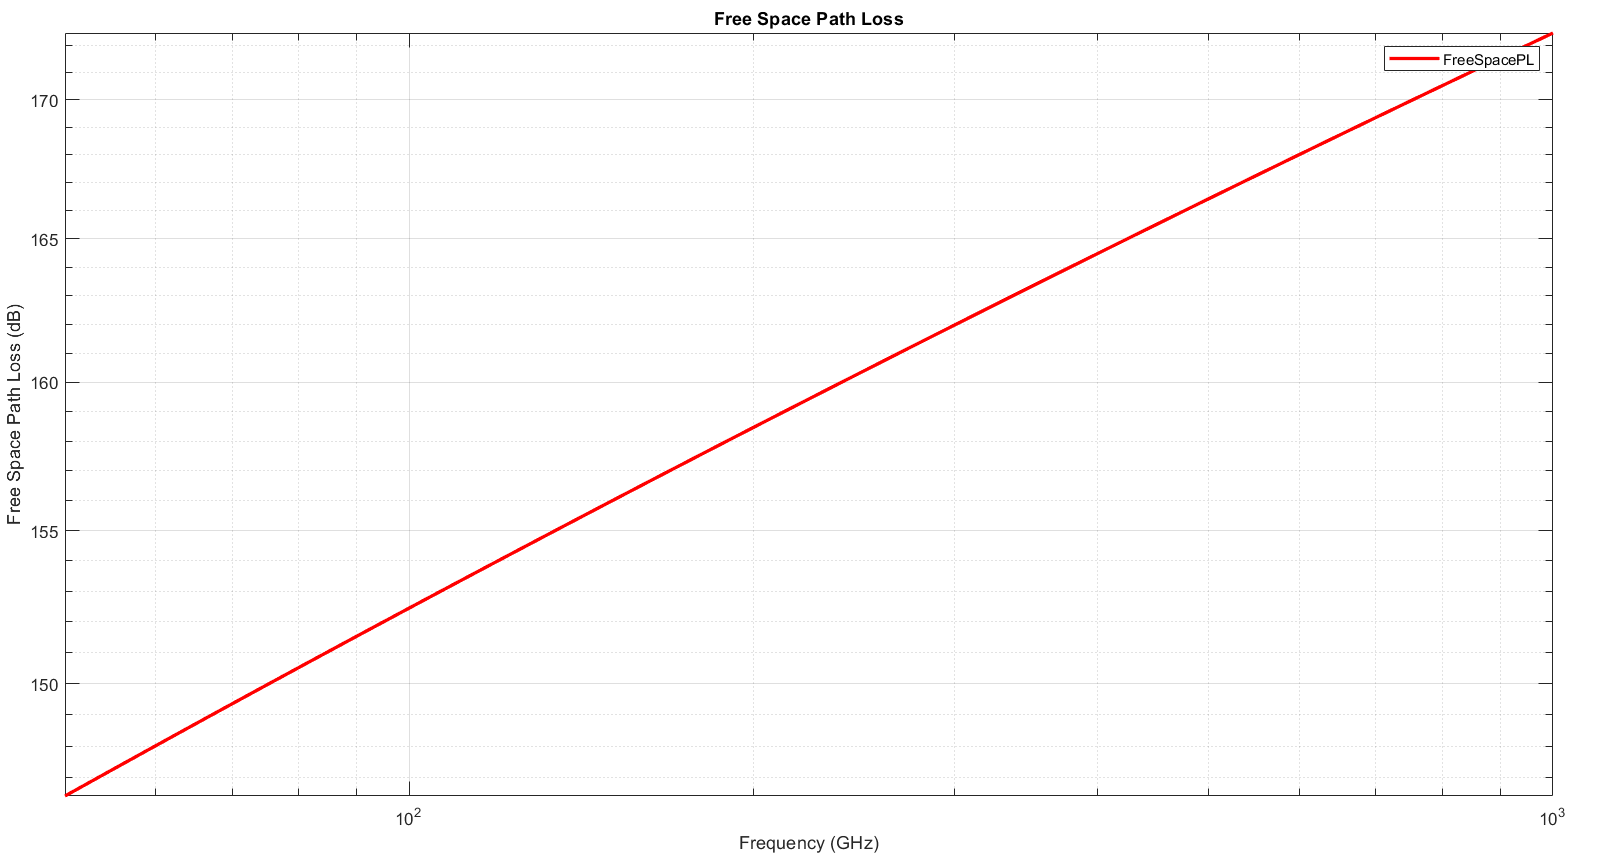
\includegraphics[scale=0.35]{figures/FreeSpacePL.png}
	\caption{Relationship between Free Space Path Loss and Frequency}
\end{figure}



%%-----------------------------------------------------------------------
\pagebreak
\subsection{Rain attenuation, Fog attenuation and Atmospheric gas attenuation with Frequency}

\textit{Note : For the generation of following plots three of the Matlab built-in functions, namely \textbf{rainpl()\cite{matlab}, gaspl()\cite{matlab}, fogpl()\cite{matlab}} which are developed according to the ITU-R P Series recommendations were used and links for their documentations are given at the Reference section.}


\subsubsection{Rain attenuation - Recommendation ITU-R P.838-3, 2005\cite{rain}}
The following plot shows how losses due to rain varies with frequency. The plot assumes the followings in addition to the provided information in the Task 1.\\

\begin{tabular}{l l}
Elevation angle of the propagation path& = 0 \\
Polarization tilt angle of the signal &= 0\\
\end{tabular}\\

In general, horizontal polarization represents the worse case for propagation loss due to rain.

\begin{figure}[!h]
	\centering
	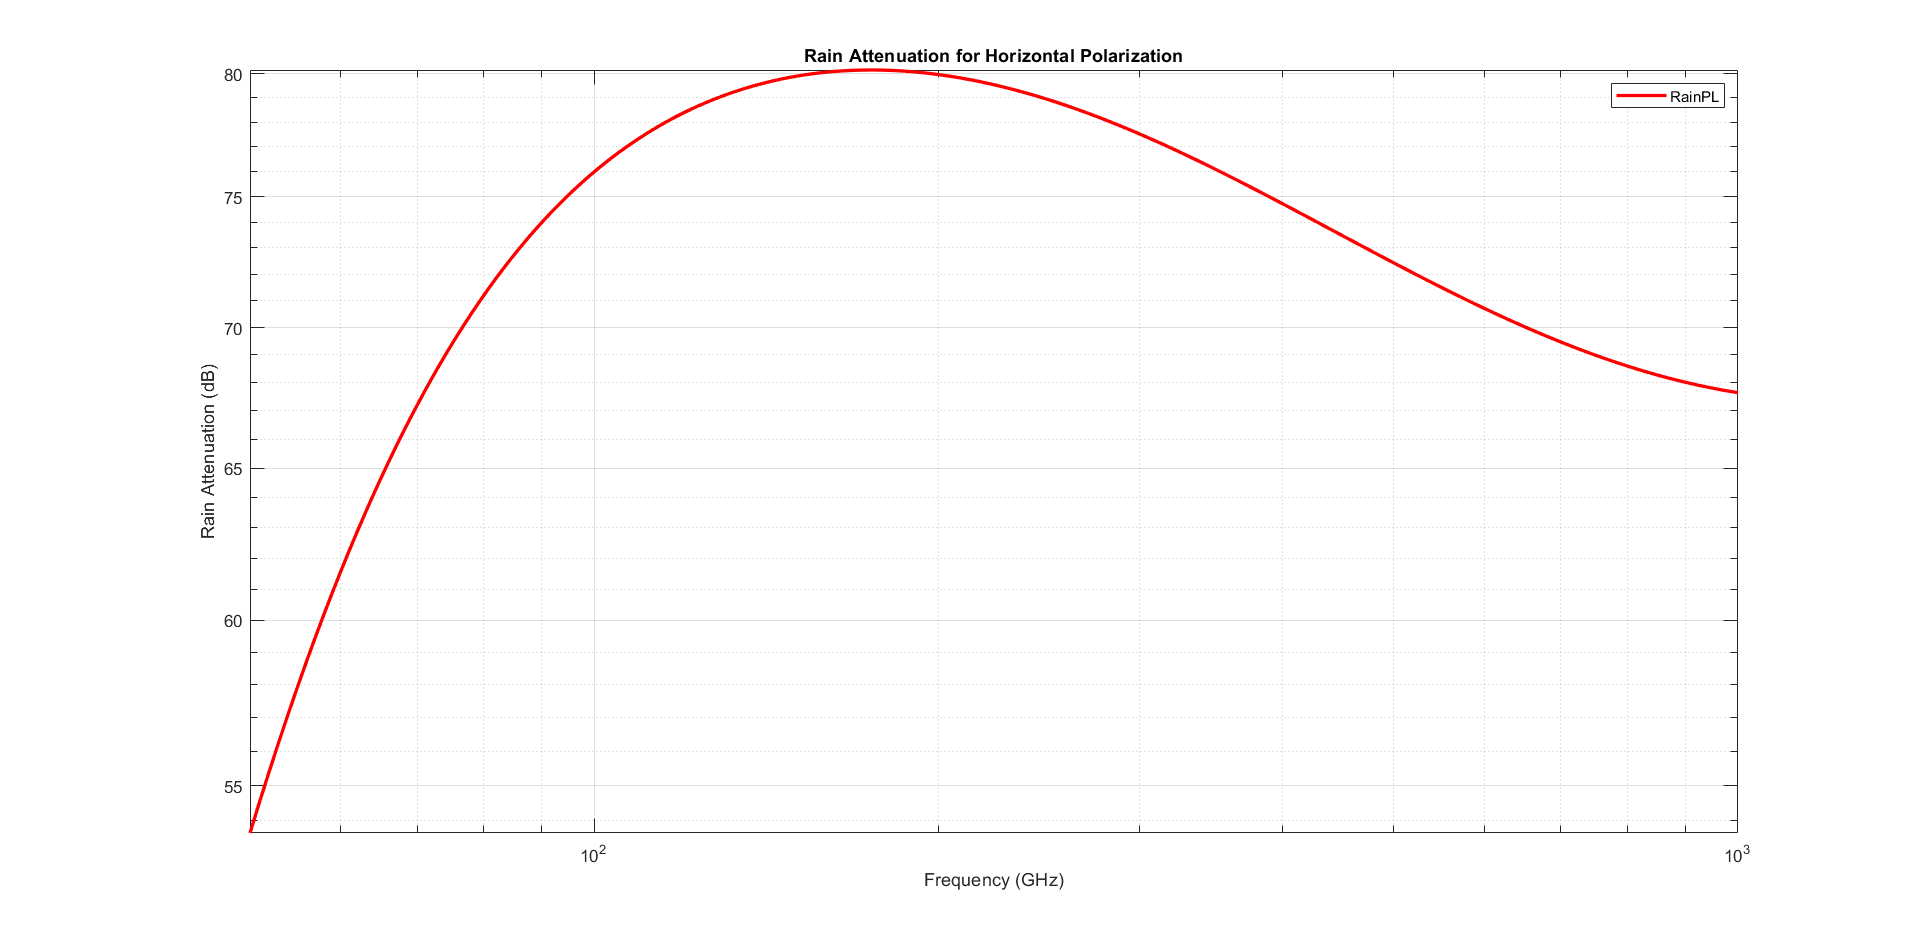
\includegraphics[scale=0.35]{figures/RainPL.png}
	\caption{Relationship between Rain attenuation and Frequency}
\end{figure}

\subsubsection{Fog attenuation - Recommendation ITU-R P.840-3, 2013\cite{fog}}
The following plot shows how losses due to fog/cloud varies with frequency. The plot assumes the following provided information in the Task 1.\\

\begin{tabular}{l l}
	Ambient Temperature in Celsius&= 31\\
	Liquid Water Density in $g/m^3$&= 0.5\\
\end{tabular}\\

\begin{figure}[!h]
	\centering
	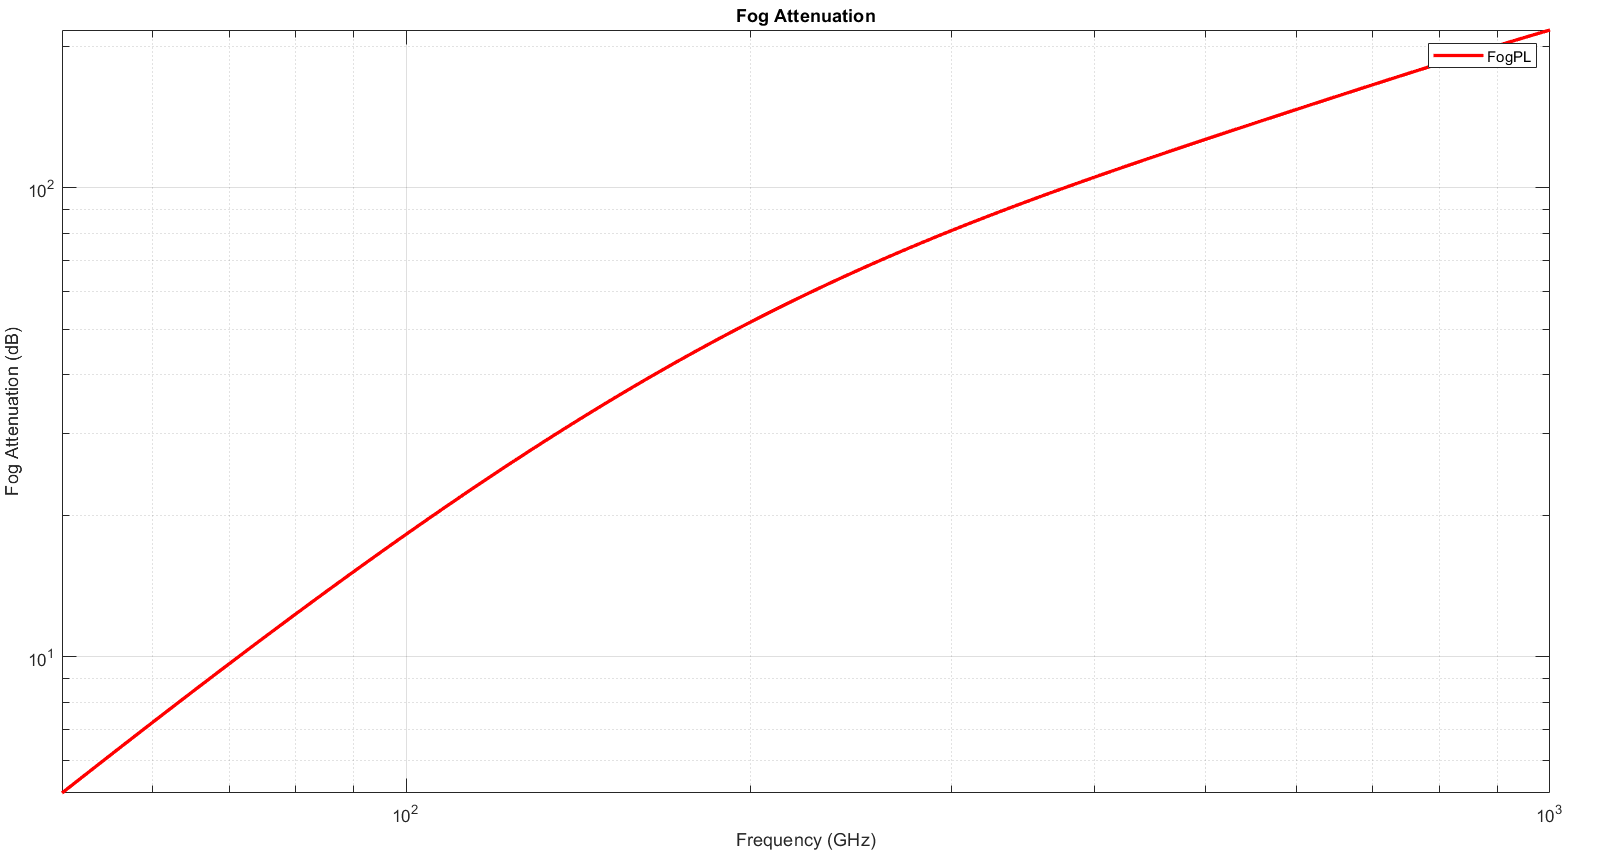
\includegraphics[scale=0.35]{figures/FogPL.png}
	\caption{Relationship between Fog attenuation  and Frequency}
\end{figure}

\subsubsection{Atmospheric gas attenuation - Recommendation ITU-R P.676-10, 2013\cite{gas}}

The plot below shows how the propagation loss due to atmospheric gases varies with the frequency. The plot assumes the followings in addition to the provided information in the Task 1.

\begin{tabular}{l l}
	 Dry air pressure in Pa&= 101325\\
	 Water Vapor Density in $g/m^3$&= 30.4\cite{vapor}\\
\end{tabular}


\begin{figure}[!h]
	\centering
	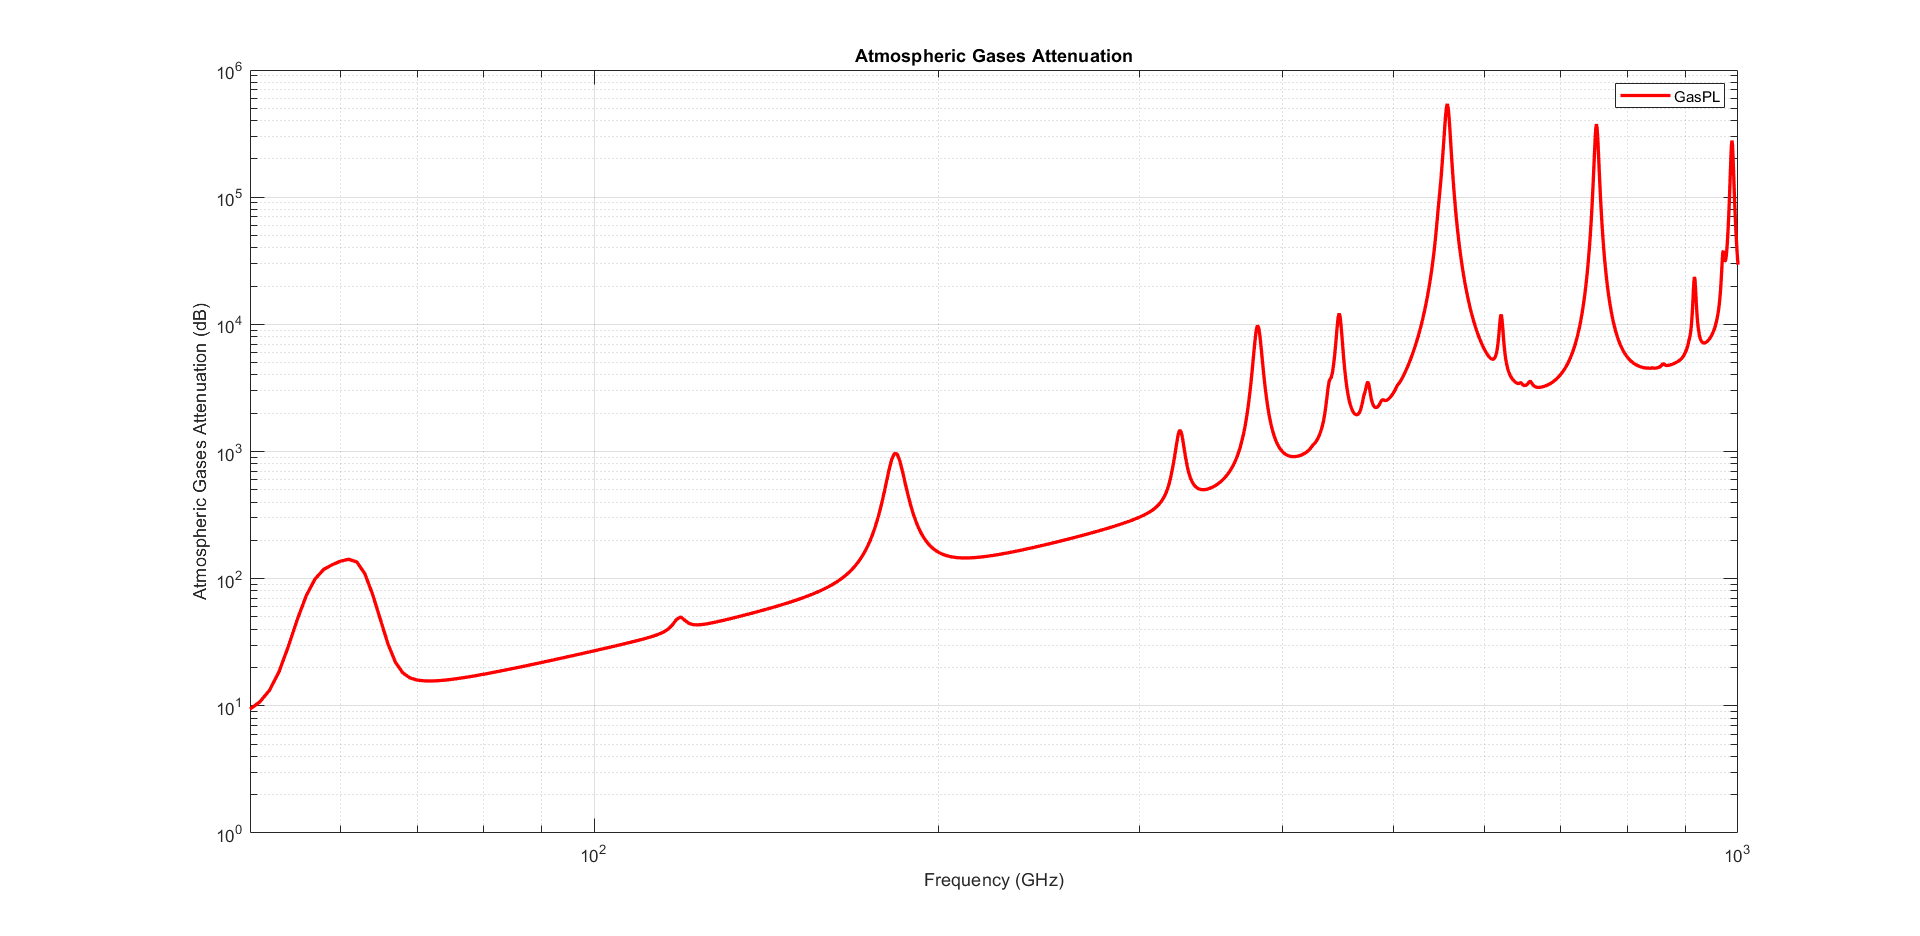
\includegraphics[scale=0.35]{figures/GasPL.png}
	\caption{Relationship between Atmospheric gas attenuation and Frequency}
\end{figure}


%%-----------------------------------------------------------------------
\subsection{Total Path Loss with Frequency}
\textit{Note : Range of frequency was chosen from 50 GHz to 1000 GHz since some of the ITU-R models are only defined in 10 GHz - 1000 GHz range.}
\begin{figure}[!h]
	\centering
	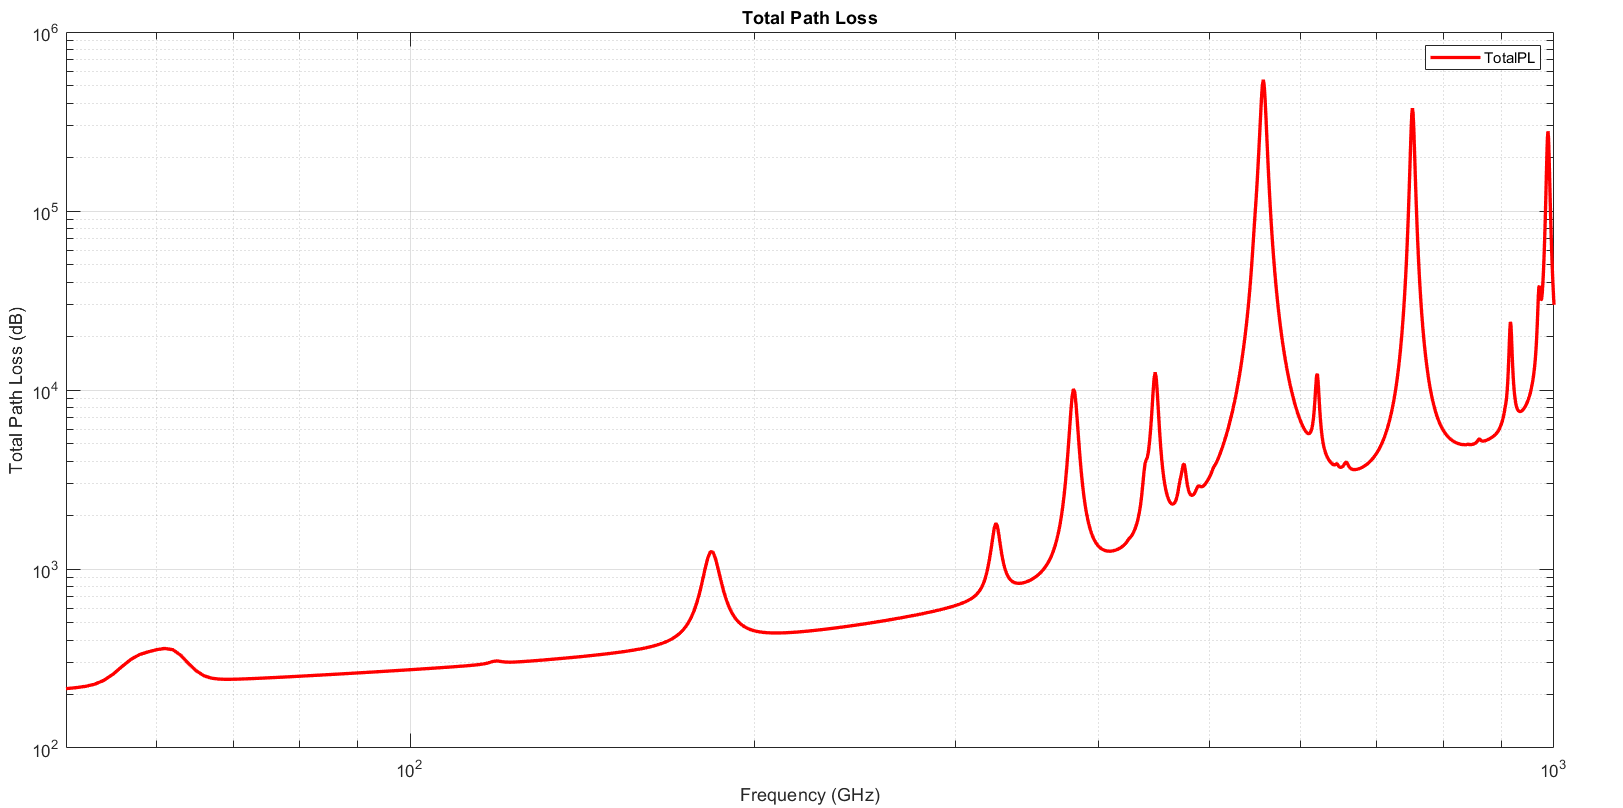
\includegraphics[scale=0.35]{figures/TotalPL.png}
	\caption{Relationship between Total Path Loss and Frequency}
\end{figure}

By inspecting the figure we can conclude that the minimum propagation loss is given at the frequency of 50 GHz in the given range. Therefore from this point onward, for the calculations it will be the frequency for transmission.\\

Minimum Propagation Loss = 214.624 dB\\
Corresponding Frequency = 50 GHz\\



\begin{figure}[!h]
	\centering
	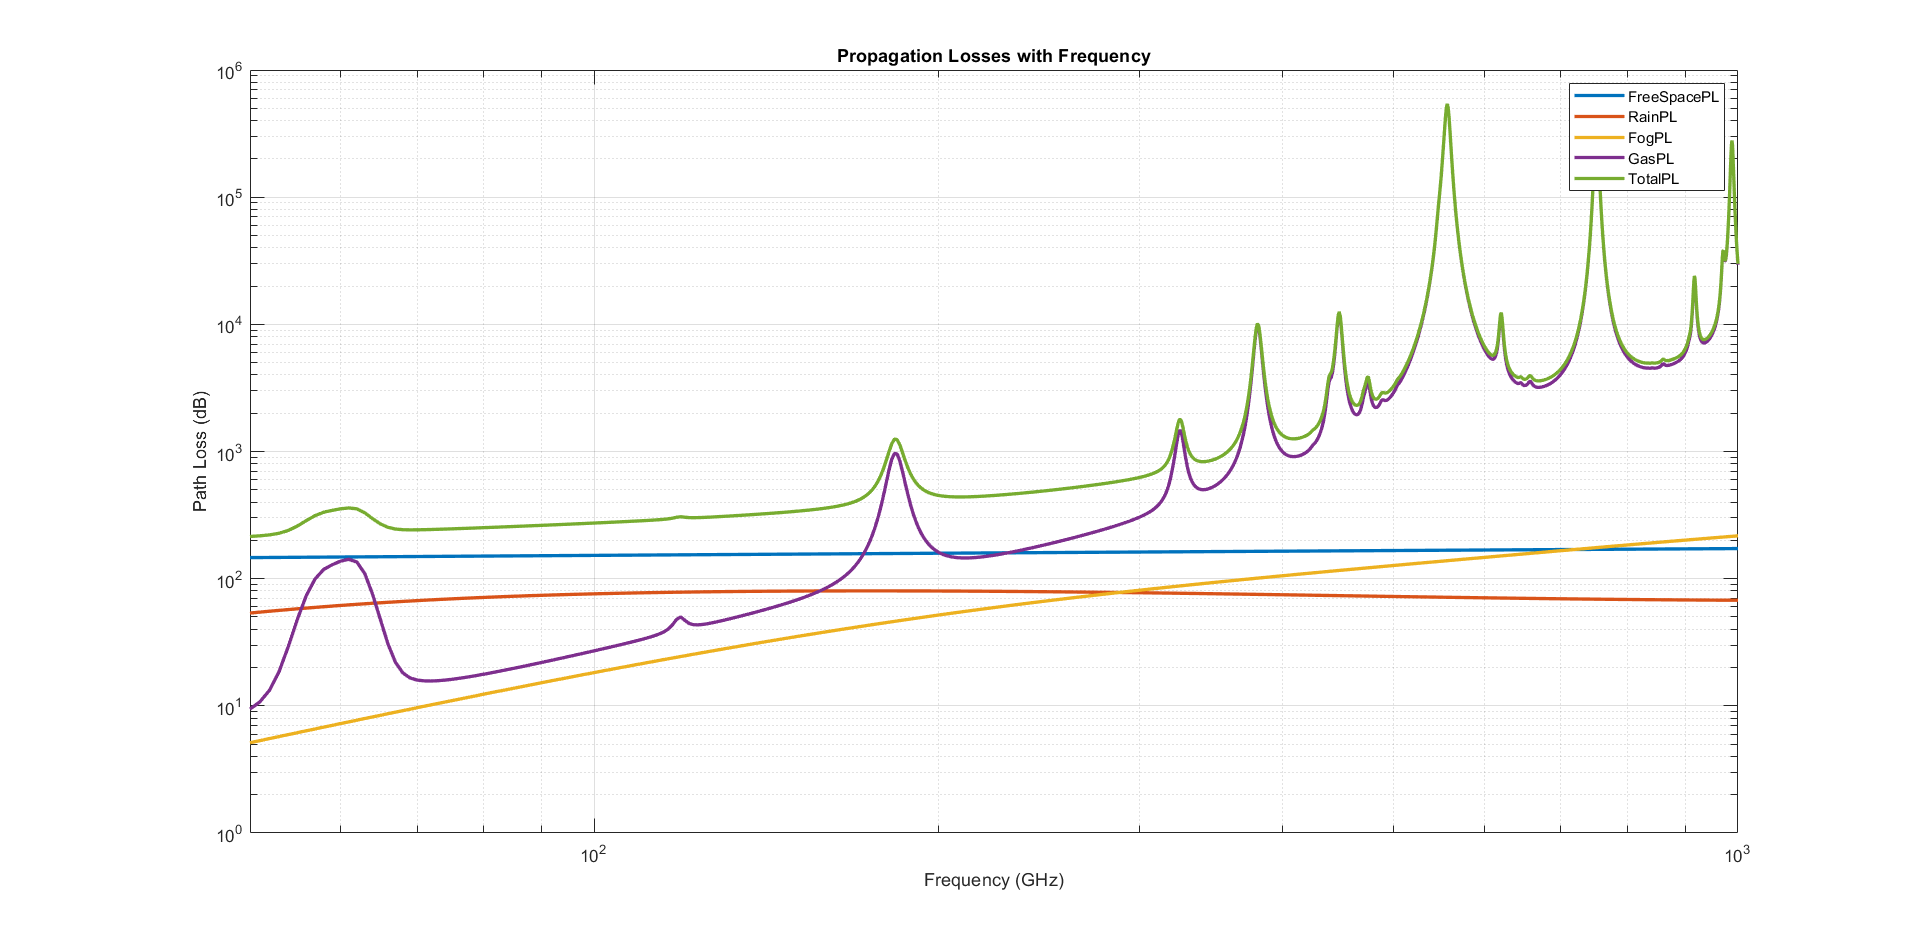
\includegraphics[scale=0.35]{figures/AllinOne.png}
	\caption{Relationship between Various Path Losses and Frequency - All in One}
\end{figure}
%\subsection{Link Budget Calculation}
%
%Parameters For the propagation model
%\begin{tabular}{l r}
%Chosen transmission frequency & 10 GHz\\
%Total Path Loss & 136.9 dB\\
%Transmission power & 50 kW or 47 dB\\
%Transmitter Gain & 30 dB\\
%Receiver Gain &24.77 dB\\
%Link margin  &11 dB\\
%Cable loss at Transmitter & 3 dB\\
%Cable loss at Receiver &4 dB\\
%\end{tabular}\\[1cm]
%
%Let's find the actual received power at the receiver\\
%
%\begin{tabular}{|l l| r|}
%	\hline
%Received Power =	&Transmission power & +47 dB\\
%&	Cable loss at Transmitter & -3 dB\\
%&	Transmitter Gain & 30 dB\\
%&	Total Path Loss & -136.9 dB\\
%&	Receiver Gain &+24.77 dB\\
%&	Cable loss at Receiver &-4 dB\\\hline
%Received Power =&&-42.13 dB\\\hline\hline
%\end{tabular}\\[1cm]
%
%
%Therefore,\\
%\begin{center}
%	\begin{tabular}{l c c c}
%Link margin  & =& Received Power& - Receiver Sensitivity\\
%11 dB& = &-42.13 dB& - Receiver Sensitivity\\
%Receiver Sensitivity &= &-53.13 dB& \\\hline\hline
%	\end{tabular}
%\end{center}

\pagebreak
\subsection{Variation of the Signal Power with the Distance}

Parameters For the propagation model\\

\begin{tabular}{l r}
Chosen Carrier frequency & 50 GHz\\
Transmission power & 50 kW or 47 dB\\
Cable loss at Transmitter & 3 dB\\
Transmitter Gain & 30 dB\\
Receiver Gain &24.77 dB\\
Cable loss at Receiver &4 dB\\
Total Path Loss & Varies with Distance\\
\end{tabular}\\[1cm]

According to above values, Let's calculate the Power of the signal when leaving the  Transmission antenna, say $P_{dB}(0~km)$,

\[
\begin{split}
P_{dB}(0~km) & = Transmission~power -  Cable~loss~at~Transmitter + Transmitter~Gain\\
&=47-3+30\\
&=74~dB
\end{split}
\]

Free Space Path Loss in dB, $L_{dB}$ as a function of distance in kilo meters. By substituting $f_{GHz}$ = 50 to the equation derived in part 1.

\[
\begin{split}
L_{dB}(d_{km})&= +92.44778322+20.\log_{10}(50) + 20.\log_{10}(d_{km})\\
&=+92.44778322+ 33.97940009 + 20.\log_{10}(d_{km})\\
&=+126.4271833+ 20.\log_{10}(d_{km})\\
\end{split}
\]

Therefore, \[Total~Path~Loss = L_{dB}(d_{km}) + Rain~Attenuation+Fog~Attenuation+Atmospheric~Gas~Attenuation \]

Therefore the Signal Power when reaching the Receiving Antenna at $d_{km}$ distance,
\[
\begin{split}
P_{dB}(d_{km}) & =74~dB - Total~Path~Loss
\end{split}
\]

\begin{figure}[!h]
	\centering
	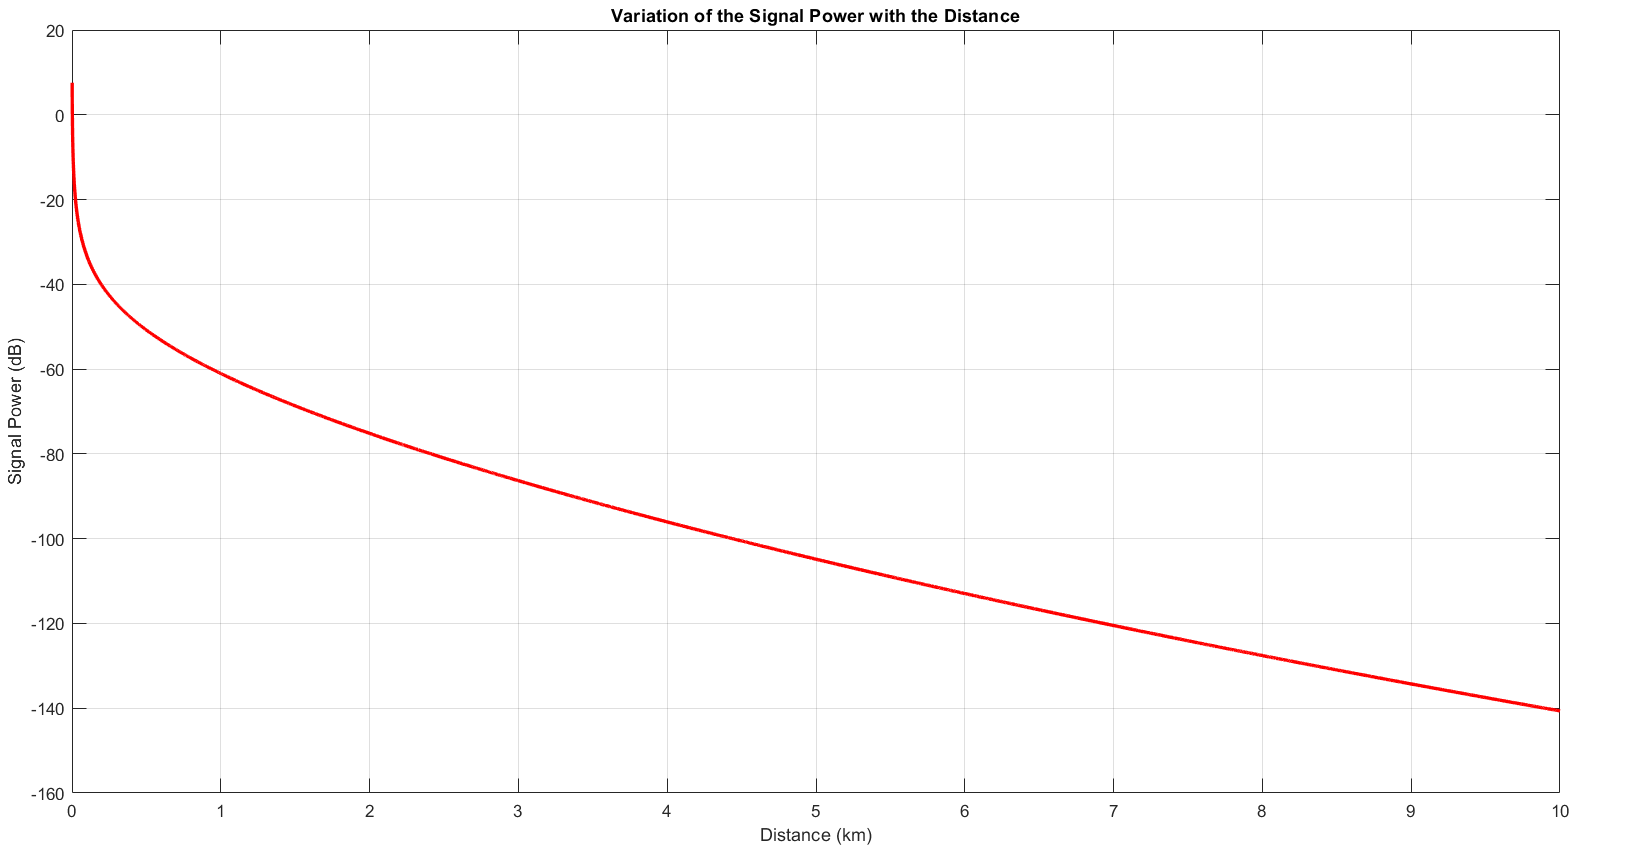
\includegraphics[scale=0.35]{figures/sp}
	\caption{Variation of the Signal Power with the Distance}
\end{figure}
\pagebreak

\subsection{Transmitting a voice signal over a noisy channel using the above Transmission frequency and the Propagation model.}
\vspace{5mm}
\subsubsection{Logic and Assumptions Used to implement the Propagation Model}

\begin{figure}[!h]
	\centering
	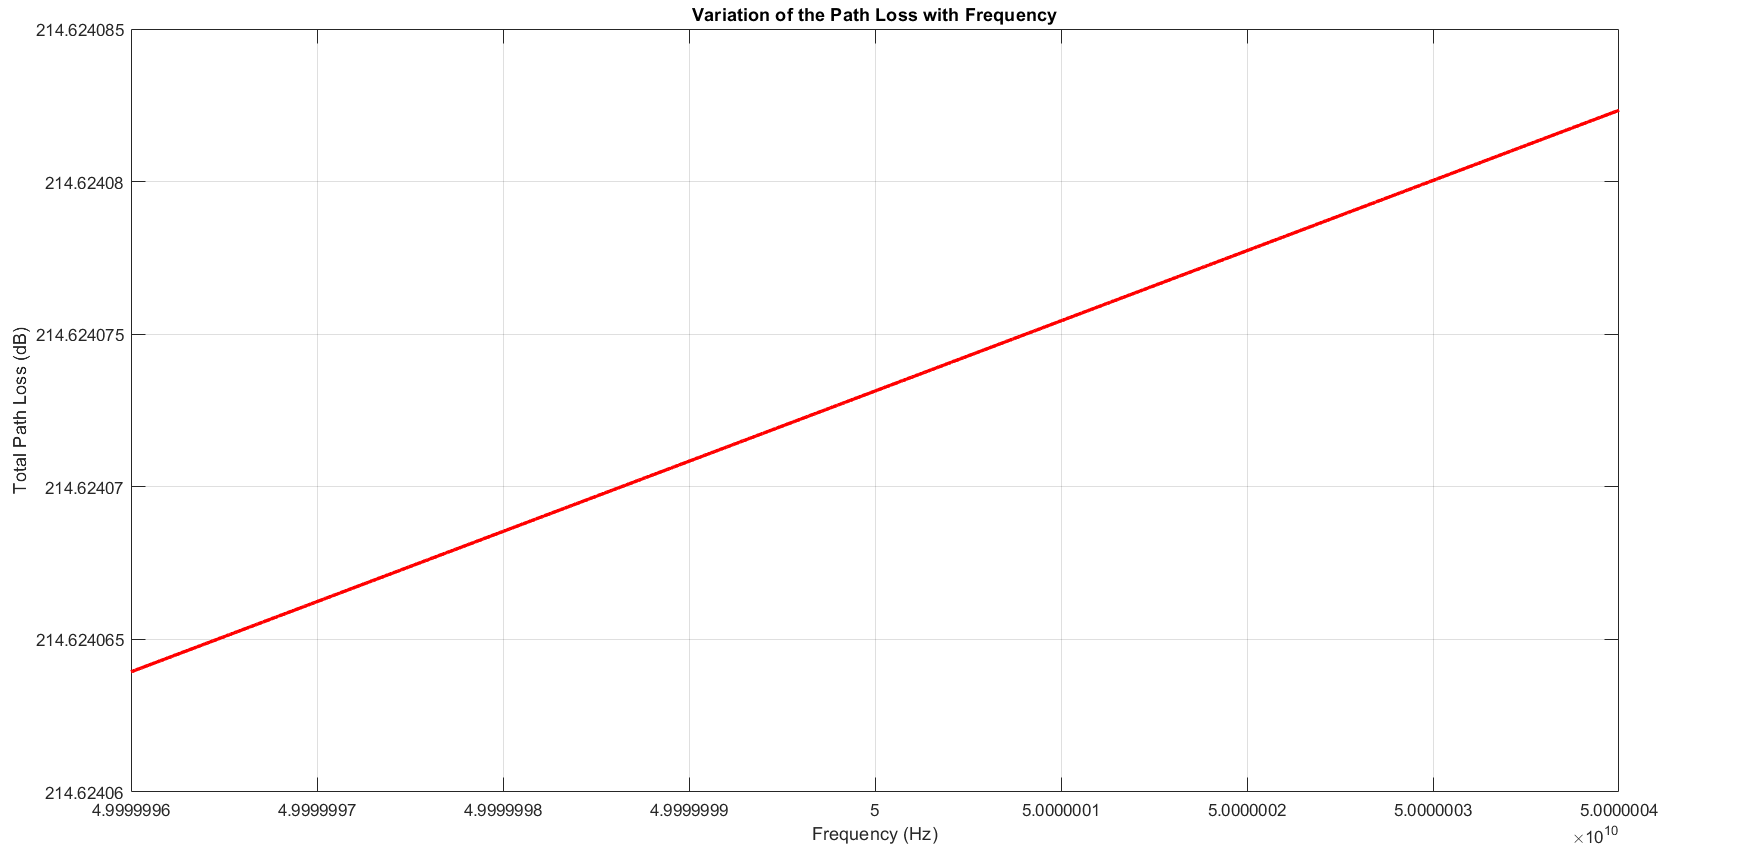
\includegraphics[scale = 0.36]{figures/voicePL}
	\caption{Variation of the Total Path Loss with the Frequency in modulated Voice Signal}
\end{figure}

By inspecting the above figure, it can be observed that the total Path Loss of the \textbf{Frequency Modulated Voice Signal}, over its frequency range( \textit{from 50e9 - 4e3 to 50e9 + 4e3})Hz changes only by a value less than 0.000025 dB which is almost Zero. Therefore in a real world application it can be assumed that the total path loss of the modulated voice signal is as same as that of the carrier wave(50 GHz) alone. That is, path loss variation due to the frequency variation in the above range can be neglected and can be assumed as a constant of 214.6240 dB which is the total path loss corresponding to the 50 GHz wave. Therefore for the following model, total path loss of the signal was taken as 214.6240 dB and it was included in the \textbf{\textit{Free Space Loss block}} .\\

In addition to that since the attenuation affects only to the amplitude of the signal, actual scenario of the Frequency Modulation of the voice signal was not considered and instead the voice signal was FM modulated using the \textbf{\textit{FM Modulator Baseband block}} which is an ideal option for simulation purposes.
\vspace{2cm}
\subsubsection{RF Propagation Model - Simulink}

Steps of the simulation are as follows:
\begin{enumerate}[1.]
	\item Input the voice.wav file of 8000Hz sampling rate using \textbf{\textit{From Multimedia File block}}.
	\item Normalization of the voice signal using \textbf{\textit{Normalization block}}.
	\item Frequency modulating the signal using \textbf{\textit{FM Modulator Baseband block}}.
	\item Addition of the -3 dB Cable loss at Transmitter using \textbf{\textit{dB Gain block}}.
	\item Addition of the 30 dB transmitter gain using the \textbf{\textit{Transmitter block}}.
	\item Addition of the effect of noise using \textbf{\textit{AWGN channel block}}.
	\item Addition of the -214.6240 dB propagation loss using \textbf{\textit{Free Space Path Loss block}}.
	\item Addition of the 24.77 dB receiver gain using  \textbf{\textit{Receiver Preamp block}}.
	\item Addition of the -4 dB Cable loss at the Receiver using \textbf{\textit{dB Gain block}}.
	\item Demodulating the signal using \textbf{\textit{FM Demodulator Baseband block}}.
	\item Saving the output voice signal using \textbf{\textit{To Multimedia File block}}.
	\item convert the output signal into audio using \textbf{\textit{Audio Device Writer block}}.
\end{enumerate}
\vspace{1cm}
Before run the simulation change the directories related to the voice input and output as mentioned in the page 1.


\begin{figure}[!h]
	\centering
	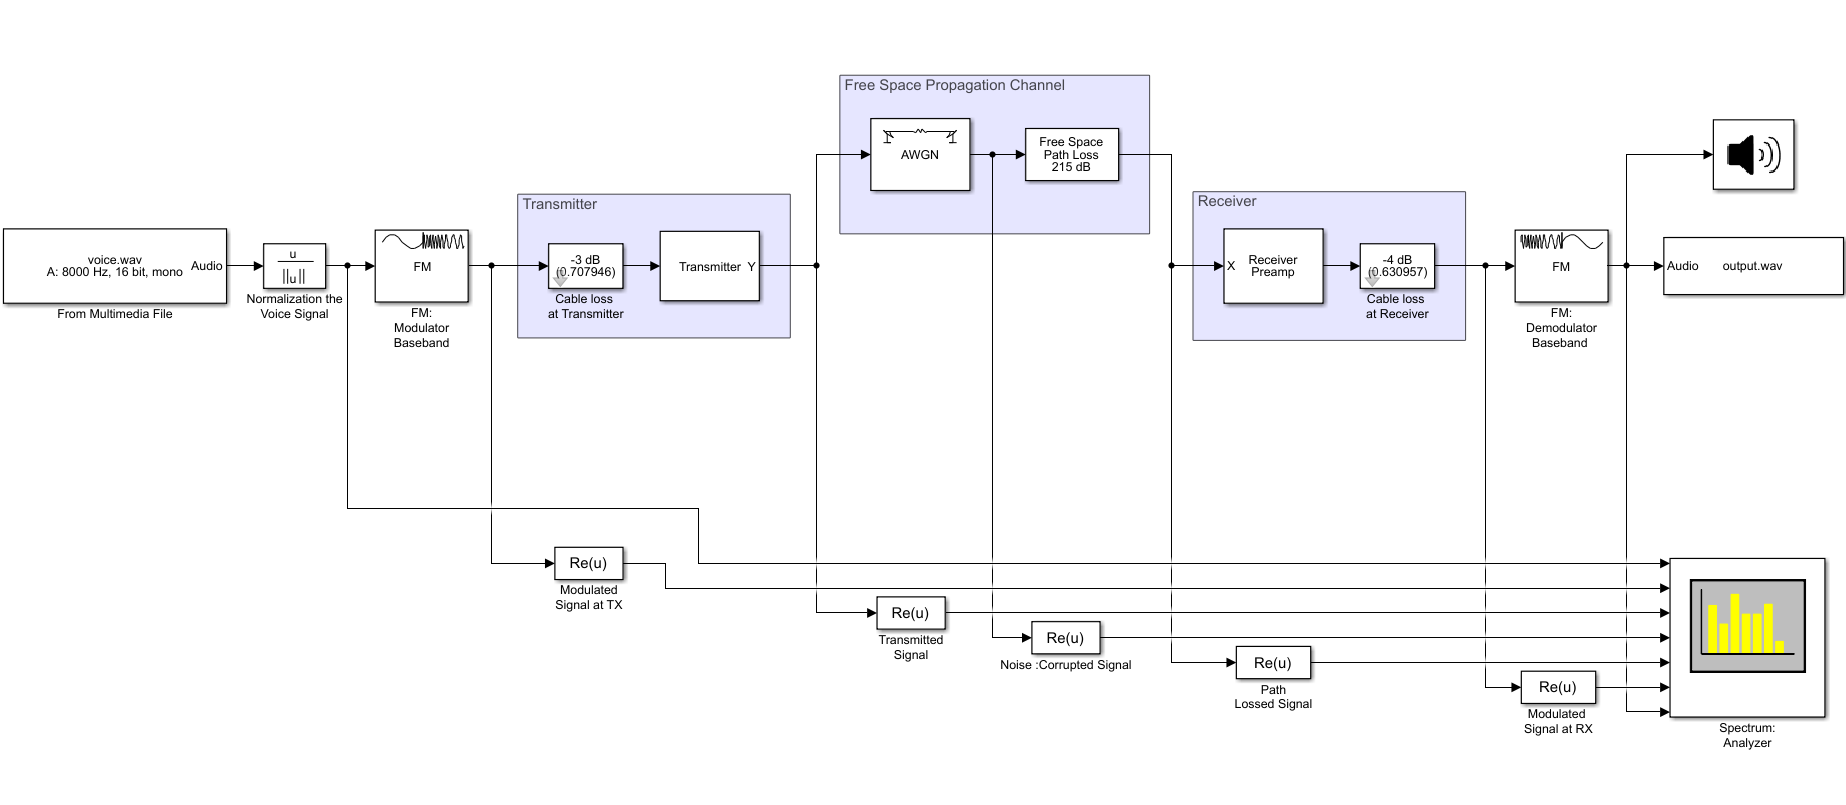
\includegraphics[scale = 0.43 ]{figures/model} %angle= 90
	\caption{RF Propagation Model - Simulink}
\end{figure}
\vspace{1.5cm}

\begin{figure}[!h]
	\centering
	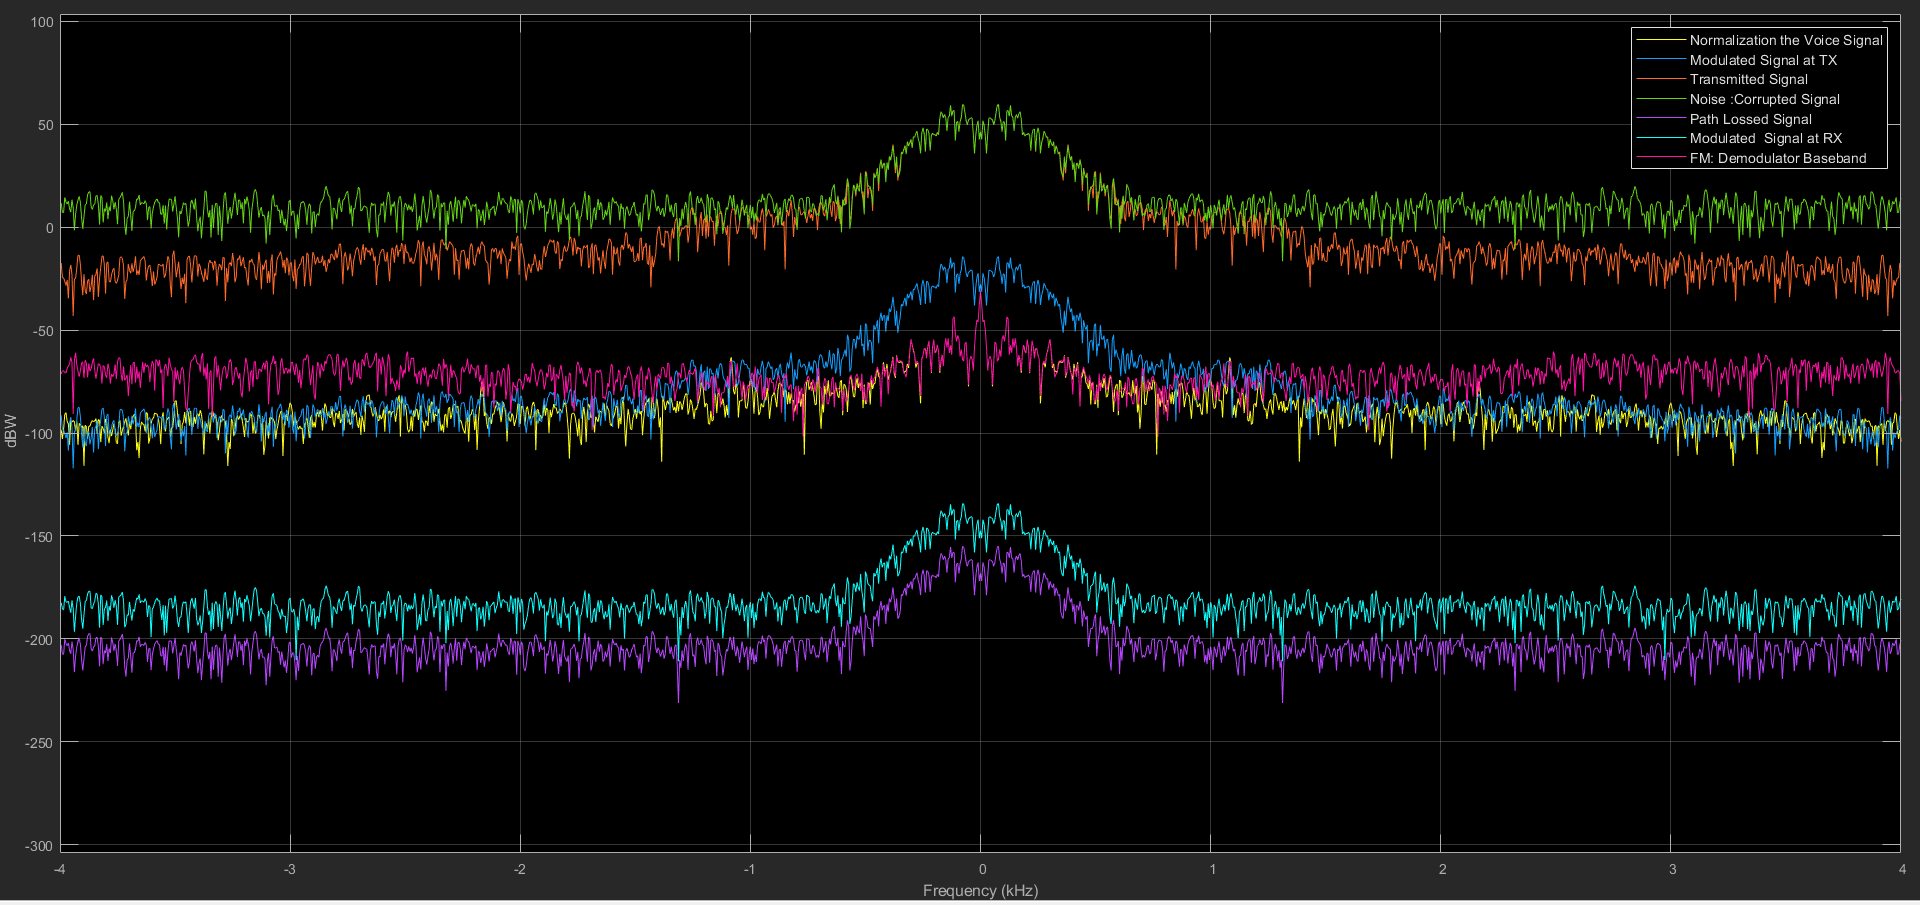
\includegraphics[scale = 0.42]{figures/spect2}
	\caption{Frequency Spectrum of the signal at Various States}
\end{figure}



\pagebreak

\subsection{Codes for Task 1}


\lstinputlisting[basicstyle = \mlttfamily\scriptsize , style = Matlab-editor]{code/RFPL.m}
\pagebreak

\lstinputlisting[basicstyle = \mlttfamily\scriptsize , style =
Matlab-editor]{code/plotCurve.m}
\vfill


%=================================TASK TWO MANET============================
\pagebreak

\section{Implementing a Simplified Version of the Dynamic Source Routing(DSR) Protocol in Ad Hoc Wireless Networks}
%%-----------------------------------------------------------------------

\subsection{Simulation of a MANET with 6 nodes}
For the simulation of the Dynamic Source Routing(DSR) Protocol, we have implemented a MANET with the aid of the code base provided in the assignment.

\subsubsection{Codes for Task 2}

We were tasked with completing the routing function in ‘node.py’ and the completed routing function is as follows.\\

\begin{python}
	"""
	    ------------------------------------------------------------------------------
	    node.py
	    ------------------------------------------------------------------------------

	"""
	def route(self, pkt):

		 if pkt.type == PKT_TYPE.RREQ:    #checking whether the packet is a
																			#route request
				 if (self.check_in_recent(pkt)) or (pkt.check_id(self.id)):
					#checking whether the packet has already passed through the node
						 self.disregard += 1  #if it has already been processed,
																	#it is counted as a disregarded packet
						 self.forward()   #proceeding onto the next packet
				 else:    #if the packet is received for the first time
						 self.add_to_recent(pkt)      #adding to the recent packet list
																					#of the node
						 if pkt.target == self.id:    #checking whether this node
																					#is the destination of the packet
								 rrepPkt = self.generate_RREP(pkt)    #creating
																											#a route reply packet
								 self.add_to_queue_out(rrepPkt)   #sending the packet
						 else:    #if the packet is not addressed to the considered node
								 pkt.add_id(self.id)     #appending the id of this node
																				 #to the packet route
								 self.add_to_queue_out(pkt)   #sending the packet

		 elif pkt.type == PKT_TYPE.RREP:  #checking whether the packet is a
																			#route reply packet
				 if pkt.source == self.id:    #checking whether the packet
																			#has reached the source
						 self.add_to_cache(pkt)   #getting the route from the packet
																			#into the cache
						 if self.check_in_buffer(pkt):    #checking whether the data
																							#packet is available in buffer
								 dataPkt = self.retrieve_from_buffer(pkt)#getting the data
																												 #packet from the
																												 #buffer(as dataPkt)
								 self.add_path_from_cache(dataPkt)    #adding the route to
																											#the data packet
								 self.add_to_queue_out(dataPkt)   #sending the packet
				 else:
						 self.add_to_queue_out(pkt)   #forwarding the route reply packet
																					#until it reaches the source

		 elif pkt.type == PKT_TYPE.DPKT:  #checking whether the packet is a
																			#data packet
				 if self.id == pkt.source:    #checking whether the packet is
																			#origintaing from the considered node
						 if self.check_in_cache(pkt): #checking for the path for
																					#the packet in the node cache
								 self.add_path_from_cache(pkt)    #adding the path from
																									#the node cache
								 self.add_to_queue_out(pkt)   #sending the packet
						 else:    #if the path for the packet is not available in cache
								 self.add_to_buffer(pkt)  #keep the data packet in a buffer
								 rreqPkt = self.generate_RREQ(pkt)    #creating a route
																											#request packet
								 self.add_to_recent(rreqPkt)  #adding the route request
																							#packet to the recents list
																							#of the node
								 self.add_to_queue_out(rreqPkt)   #sending the packet
				 elif self.id == pkt.target:  #checking whether the data packet
																			#has reached its destination
						 self.received.append(pkt)    #saving the received data packet
				 else:
							self.add_to_queue_out(pkt)
\end{python}
\vspace{1cm}
In addition, we have also created ‘results.py’ which we have used to interpret the final evaluation results of the simulation.\\

\begin{python}
	"""
	    ------------------------------------------------------------------------------
	    results.py
	    ------------------------------------------------------------------------------

	"""

	from .packet import PKT_TYPE

	class Results:
	    def __init__(self):
	        self.dpkt_count = 0
	        self.total_hops = 0
	        self.counted_dpkts = []

	    def counter(self,pkt):
	        """
	        Checking the ID of packets to avoid duplicates
	        and counting the number of data packets
	        """
	        self.total_hops += 1
	        if (pkt.id) not in (self.counted_dpkts):
	            self.counted_dpkts.append(pkt.id)
	            self.dpkt_count += 1

	    def print_results(self):
	        """
	        Printing the results
	        """
	        print ("Number of data packets :",self.dpkt_count)
	        print("Total hops :",self.total_hops)
	        print(
	            "Average no. of hops per data packet :",
	            (self.total_hops/self.dpkt_count)
	            )
\end{python}
\pagebreak
Finally, the ‘demo.py’ file which was used to run the simulation is given below.
We have used a MANET consisting of 6 nodes
We have simulated for the transmission of 4 data packets.\\

\begin{python}
	"""
	    ------------------------------------------------------------------------------
	    demo.py
	    ------------------------------------------------------------------------------

	"""

	from simulator.graph import Graph
	from simulator.visualizer import step
	import cv2

	manet = Graph()

	# initialize network

	tx_range = 200
	dynamic = False  from simulator.graph import Graph
	from simulator.visualizer import step
	import cv2

	manet = Graph()

	# initialize network


	tx_range = 200
	dynamic = False  # True to use mobile model

	no_of_hops =0

	manet.add_node(500, 550, tx_range)  # "Add node 0 at 500,500"
	manet.add_node(690, 600, tx_range)  # "Add node 1 at 690,600"
	manet.add_node(780, 700, tx_range)  # "Add node 2 at 780,700"
	manet.add_node(750, 600, tx_range)  # "Add node 3 at 750,600"
	manet.add_node(790, 500, tx_range)  # "Add node 4 at 790,500"
	manet.add_node(950, 600, tx_range)  # "Add node 5 at 950,600"

	manet.send(0, 5, 1, 'Test')  # send a data packet at time step 1
	                             # from node 0 to 5
	manet.send(4, 0, 1, 'Test')  # send a data packet at time step 1
	                             # from node 4 to 1
	manet.send(2, 0, 3, 'Test')  # send a data packet at time step 3
	                             # from node 2 to 0
	manet.send(4, 2, 7, 'Test')  # send a data packet at time step 7
	                             # from node 4 to 2
	for t in range(15):  # Simulate for 15 time steps
	    step(manet, t, dynamic)

	manet.results.print_results()

	cv2.destroyAllWindows()
\end{python}

\subsubsection{Terminal Output of the Simulation}

\begin{verbatim}
	step 00:  []

	step 01:  [('0', '1', 'REQ', ('0', '5')), ('4', '1', 'REQ', ('4', '0')),
					  ('4', '3', 'REQ', ('4', '0')), ('4', '5', 'REQ', ('4', '0'))]

	step 02:  [('1', '0', 'REQ', ('0', '5')), ('1', '2', 'REQ', ('0', '5')),
					  ('1', '3', 'REQ', ('0', '5')), ('1', '4', 'REQ', ('0', '5')),
					  ('3', '1', 'REQ', ('4', '0')), ('3', '2', 'REQ', ('4', '0')),
					  ('3', '4', 'REQ', ('4', '0')), ('5', '2', 'REQ', ('4', '0')),
					  ('5', '4', 'REQ', ('4', '0'))]

	step 03:  [('1', '0', 'REQ', ('4', '0')), ('1', '2', 'REQ', ('4', '0')),
					  ('1', '3', 'REQ', ('4', '0')), ('1', '4', 'REQ', ('4', '0')),
					  ('2', '1', 'REQ', ('0', '5')), ('2', '3', 'REQ', ('0', '5')),
					  ('2', '5', 'REQ', ('0', '5')), ('3', '1', 'REQ', ('0', '5')),
					  ('3', '2', 'REQ', ('0', '5')), ('3', '4', 'REQ', ('0', '5')),
					  ('4', '1', 'REQ', ('0', '5')), ('4', '3', 'REQ', ('0', '5')),
					  ('4', '5', 'REQ', ('0', '5'))]

	step 04:  [('0', '1', 'REP', ('4', '0')), ('2', '1', 'REQ', ('4', '0')),
					  ('2', '3', 'REQ', ('4', '0')), ('2', '5', 'REQ', ('4', '0')),
					  ('5', '2', 'REP', ('0', '5'))]

	step 05:  [('1', '4', 'REP', ('4', '0')), ('2', '1', 'REQ', ('2', '0')),
					  ('2', '3', 'REQ', ('2', '0')), ('2', '5', 'REQ', ('2', '0'))]

	step 06:  [('1', '0', 'REQ', ('2', '0')), ('1', '2', 'REQ', ('2', '0')),
					  ('1', '3', 'REQ', ('2', '0')), ('1', '4', 'REQ', ('2', '0')),
					  ('2', '1', 'REP', ('0', '5')), ('3', '1', 'REQ', ('2', '0')),
					  ('3', '2', 'REQ', ('2', '0')), ('3', '4', 'REQ', ('2', '0')),
					  ('4', '1', 'DATA', ('4', '0')), ('5', '2', 'REQ', ('2', '0')),
					  ('5', '4', 'REQ', ('2', '0'))]

	step 07:  [('0', '1', 'REP', ('2', '0')), ('1', '0', 'REP', ('0', '5')),
					  ('4', '1', 'REQ', ('2', '0')), ('4', '3', 'REQ', ('2', '0')),
					  ('4', '5', 'REQ', ('2', '0')), ('5', '2', 'REQ', ('5', '2')),
					  ('5', '4', 'REQ', ('5', '2'))]

	step 08:  [('0', '1', 'DATA', ('0', '5')), ('1', '0', 'DATA', ('4', '0')),
					  ('2', '5', 'REP', ('5', '2')), ('4', '1', 'REQ', ('5', '2')),
					  ('4', '3', 'REQ', ('5', '2')), ('4', '5', 'REQ', ('5', '2'))]

	step 09:  [('1', '2', 'REP', ('2', '0')), ('3', '1', 'REQ', ('5', '2')),
					  ('3', '2', 'REQ', ('5', '2')), ('3', '4', 'REQ', ('5', '2')),
					  ('5', '2', 'DATA', ('5', '2'))]

	step 10:  [('1', '2', 'DATA', ('0', '5')), ('2', '1', 'DATA', ('2', '0'))]

	step 11:  [('1', '0', 'REQ', ('5', '2')), ('1', '2', 'REQ', ('5', '2')),
						 ('1', '3', 'REQ', ('5', '2')), ('1', '4', 'REQ', ('5', '2'))]

	step 12:  [('0', '1', 'REQ', ('5', '2')), ('1', '0', 'DATA', ('2', '0')),
					   ('2', '5', 'DATA', ('0', '5'))]

	step 13:  []
	step 14:  []
\end{verbatim}
\pagebreak

\subsubsection{Visualizer Outputs}

\begin{figure}[!h]
	\centering
	\subfigure[Step 0]
	{ 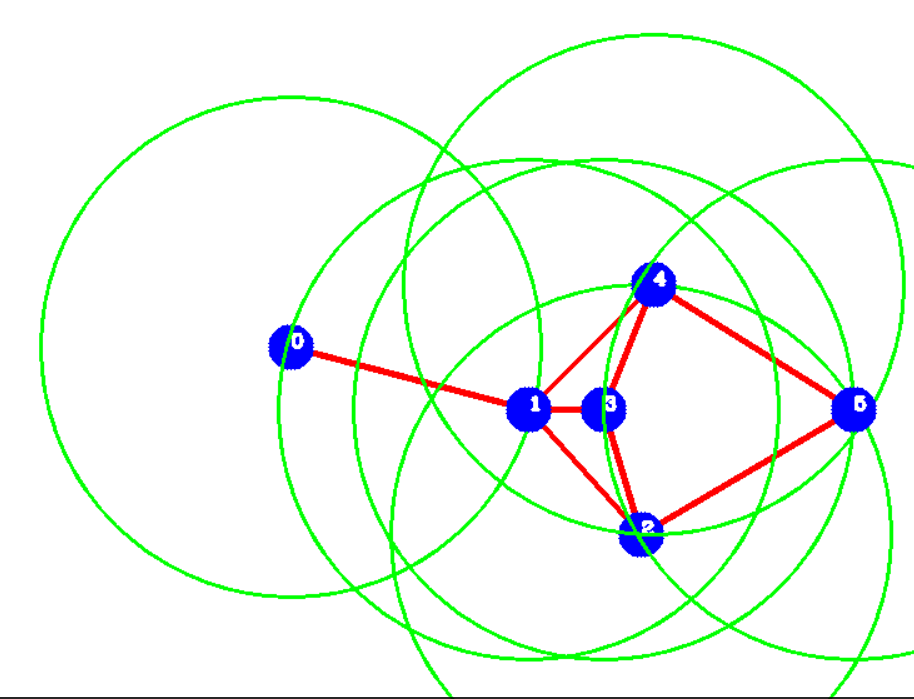
\includegraphics[scale=0.165]{figures/outputs/step_0.png}

	}\hfill
	\subfigure[Step 1]
	{ 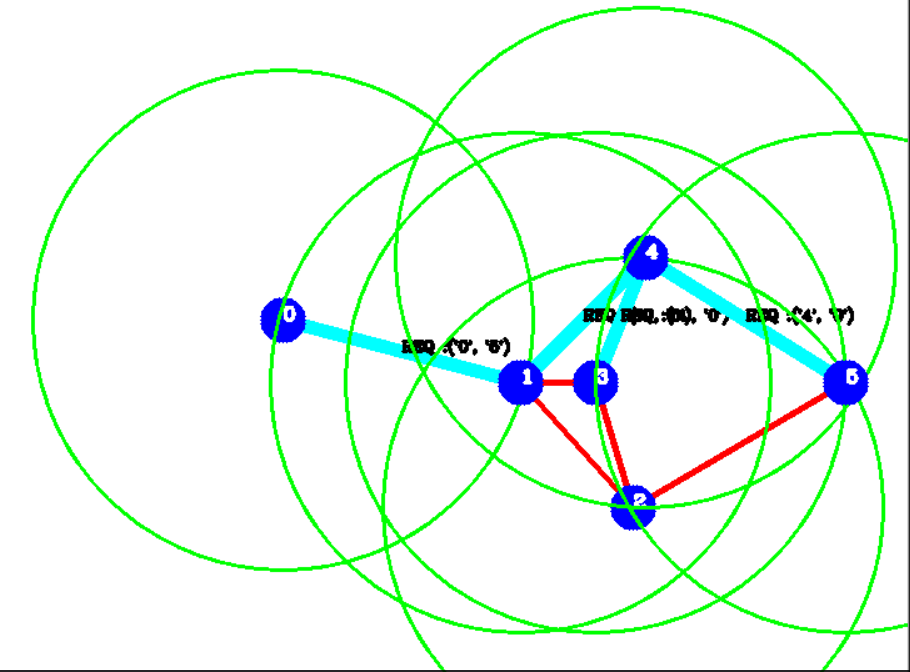
\includegraphics[scale=0.165]{figures/outputs/step_1.png}

	}\hfill
	\subfigure[Step 2]
	{ 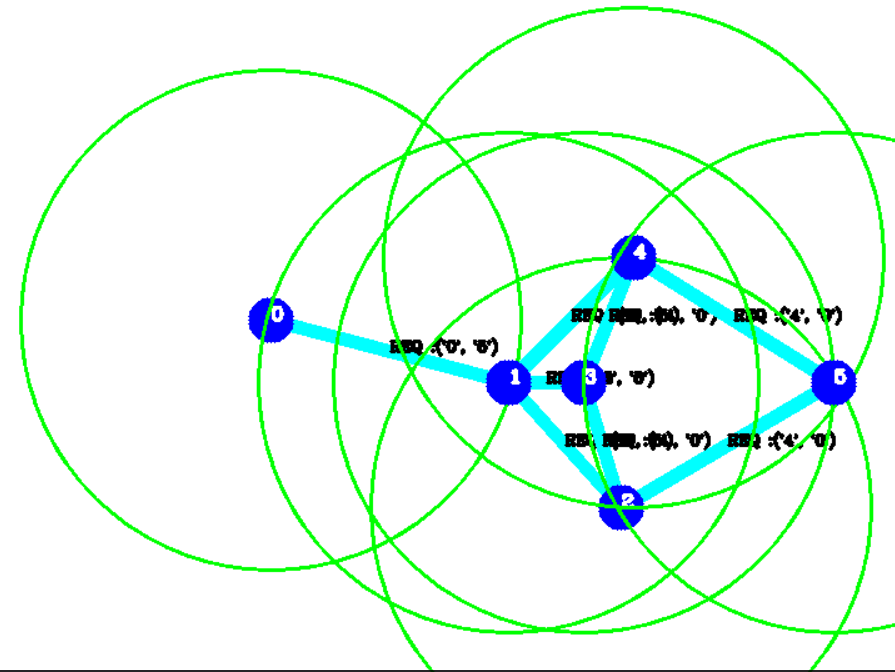
\includegraphics[scale=0.165]{figures/outputs/step_2.png}
	}\\
	\subfigure[Step 3]
	{ 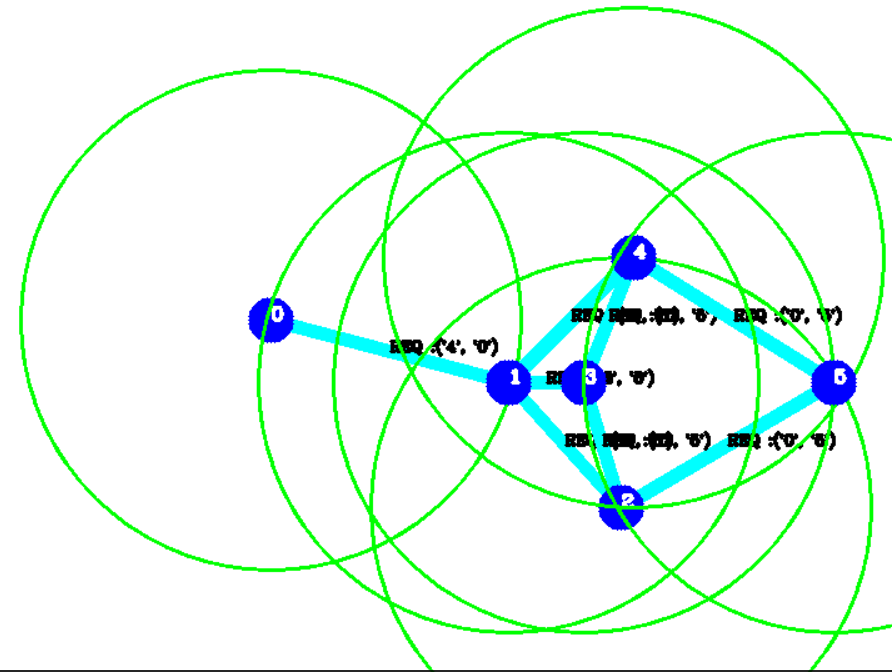
\includegraphics[scale=0.165]{figures/outputs/step_3.png}

	}\hfill
	\subfigure[Step 4]
	{ 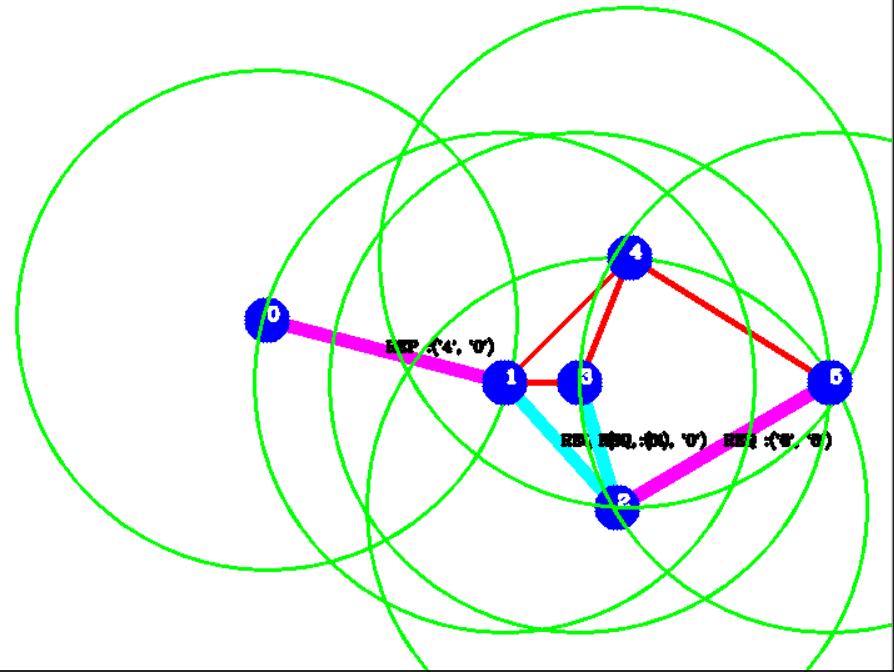
\includegraphics[scale=0.165]{figures/outputs/step_4.png}

	}\hfill
	\subfigure[Step 5]
	{ 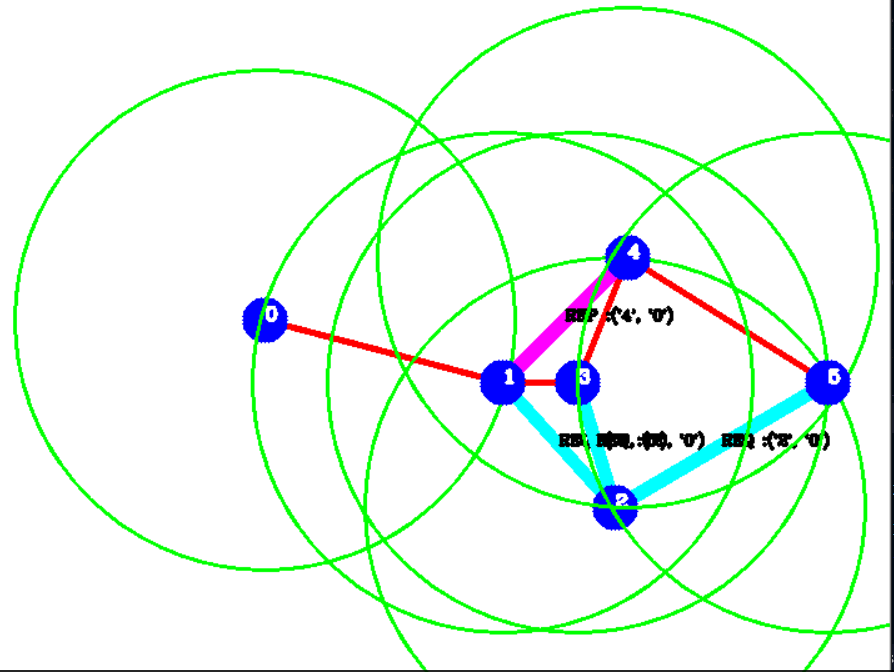
\includegraphics[scale=0.165]{figures/outputs/step_5.png}
	}\\

	\subfigure[Step 6]
	{ 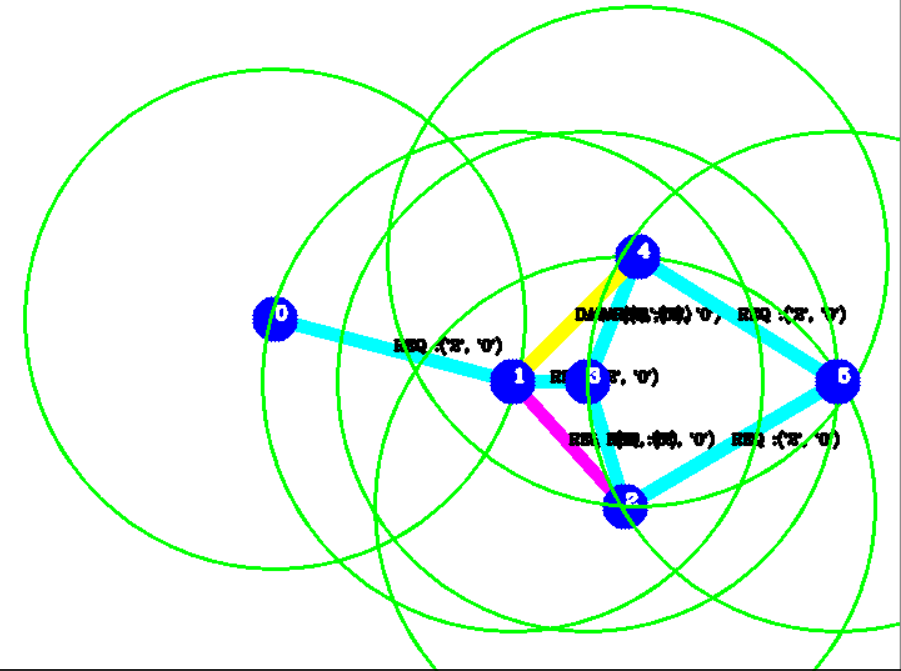
\includegraphics[scale=0.165]{figures/outputs/step_6.png}

	}\hfill
	\subfigure[Step 7]
	{ 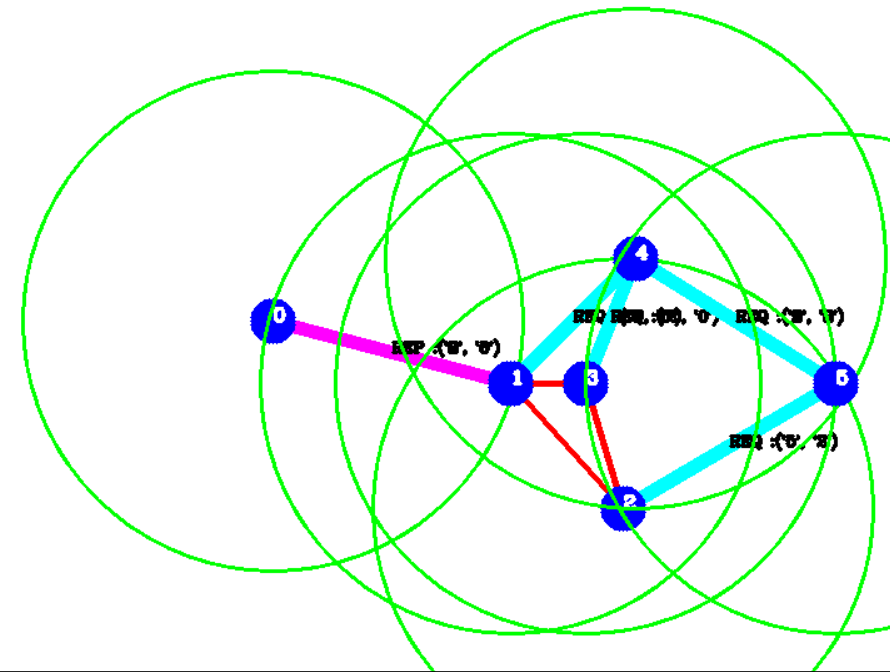
\includegraphics[scale=0.165]{figures/outputs/step_7.png}

	}\hfill
	\subfigure[Step 8]
	{ 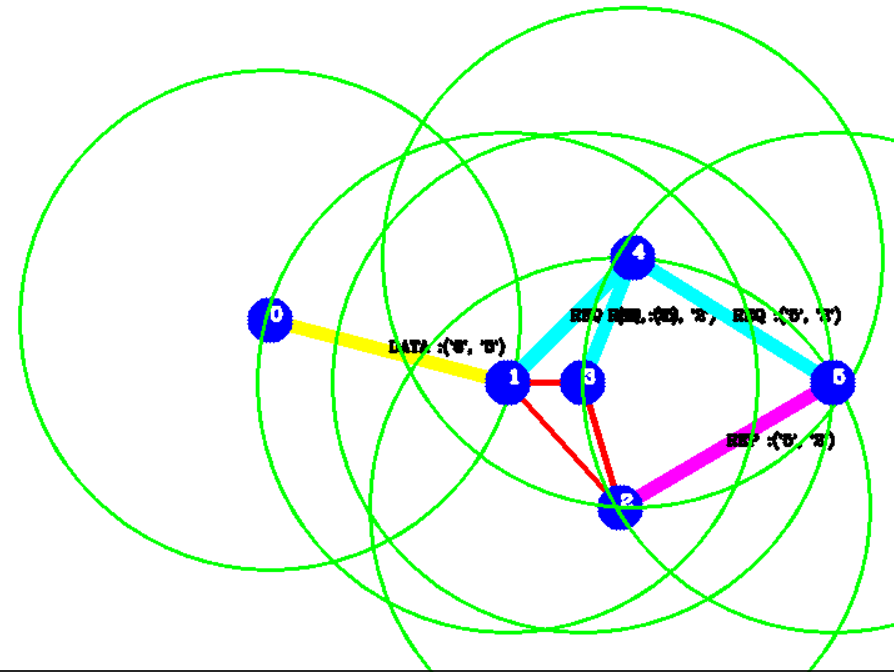
\includegraphics[scale=0.165]{figures/outputs/step_8.png}
	}\\

	\subfigure[Step 9]
	{ 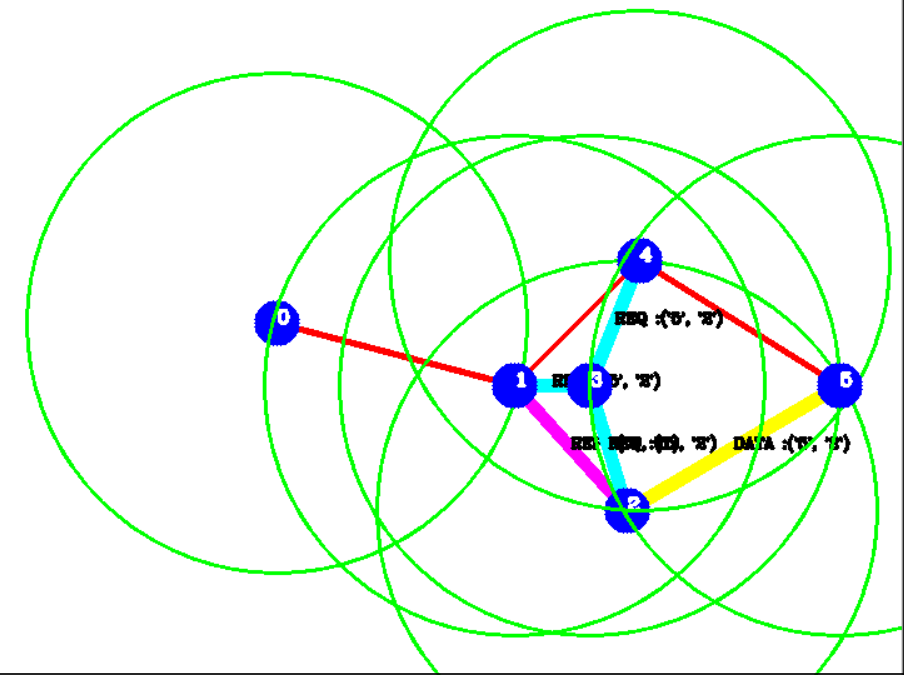
\includegraphics[scale=0.165]{figures/outputs/step_9.png}

	}\hfill
	\subfigure[Step 10]
	{ 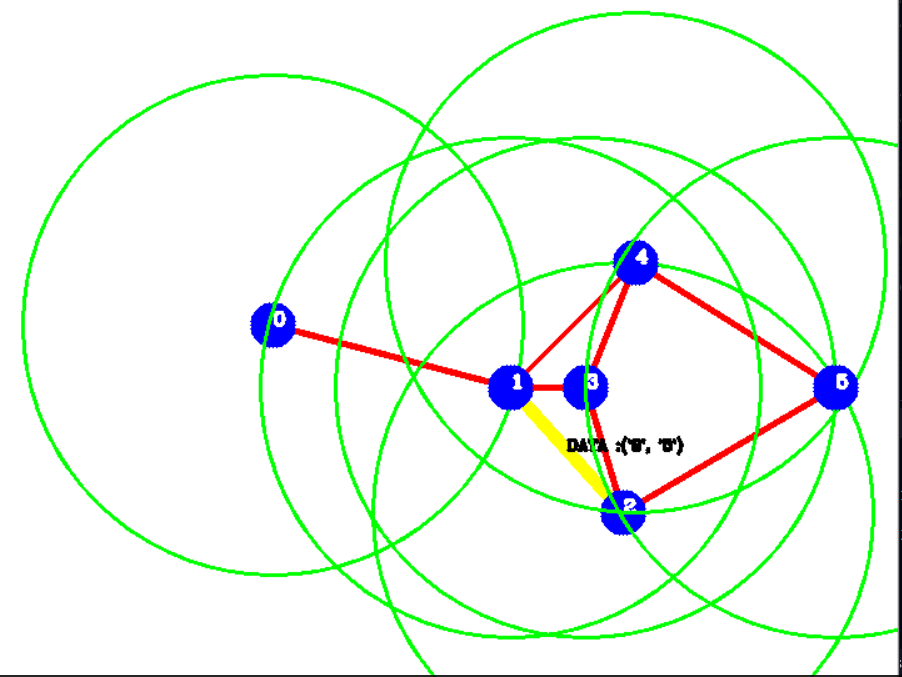
\includegraphics[scale=0.165]{figures/outputs/step_10.png}

	}\hfill
	\subfigure[Step 11]
	{ 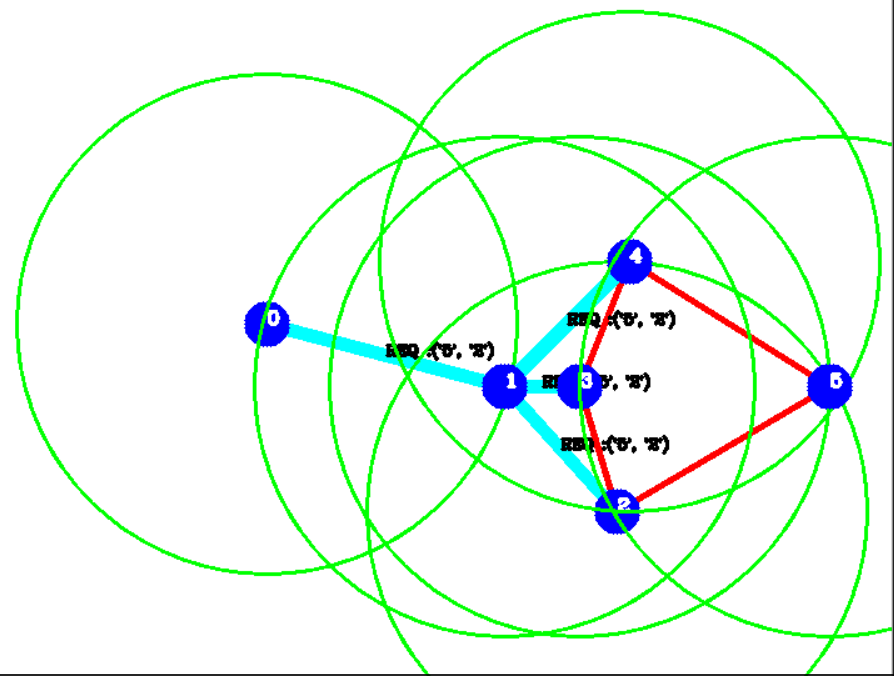
\includegraphics[scale=0.165]{figures/outputs/step_11.png}

	}\hfill
	\subfigure[Step 12]
	{ 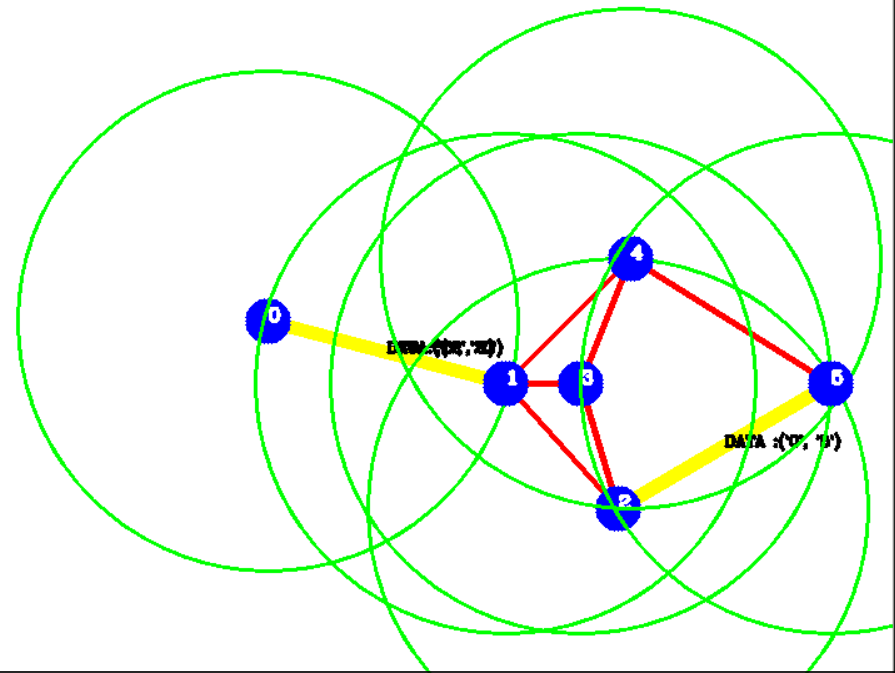
\includegraphics[scale=0.165]{figures/outputs/step_12.png}

	}\\
	\caption{The visualizer outputs for each time step}
	%\label{}
\end{figure}


\textbf{The results of the final evaluation is as follows.}\\

Number of data packets : 4\\
Total hops : 8\\
Average no. of hops per data packet : 2.0\\


%---------------------------------------------------------------------------


\subsection{Improving the Efficiency of Protocol by further Exploiting the Route Cache}

\subsubsection{Derestricting route format}
In the existing system, the entries in the route cache contain a specific format as [(target : route), (target : route) ..].
This generates the following inefficiency.
\begin{figure}[!h]
	\centering
	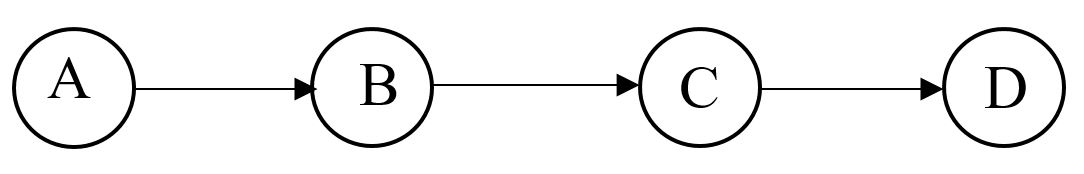
\includegraphics[scale = 0.4]{figures/route}
	\caption{A Route which is already in the Route Cache}
\end{figure}

Consider an instance where a packet has to be sent from node A to node C and also assume that the route to node D also exists in the route cache of A as (D : B, C, D)
The node A is unable to extract the route to node C from this entry as node C is not listed as the target node. Instead another route reply packet has to be initiated to find the path to node C.
If this format is derestricted and used in a manner such that the path to a node inside any entry can be extracted, the number of route request transmissions can be minimized, hence propagation time as well as CPU overhead required to process those packets is reduced.

\subsubsection{Intermediate nodes resolving a route request using their route caches}
In the existing system, once a node receives a route request, it checks to see if it is the target node for that packet and if not, it broadcasts the route request packet again.
As an alternative, once a node receives a route request, the following algorithm can be implemented.

\begin{verbatim}
IF packet ID already processed
   THEN skip packet
ELSE
   add packet ID to the recents list
   IF current node is target node
      THEN append current node ID to path and initiate RREP
   ELSE IF the path to destination exists in the routing cache of current node
      THEN append that route to path and initiate RREP
   ELSE
      append current node ID to path and broadcast
\end{verbatim}

This will enable the system to minimize route request transmissions.
However, steps have to be taken to avoid processing multiple route reply packets from multiple nodes and to select the shortest path among them.

\subsection{Handling Disconnections During Transmission}


To make the process of handling disconnections more robust, we propose that an acknowledgement message be sent during each transmission. For example, in a situation where a data packet is to be sent from node A to node D using the path A-B-C-D,
\begin{enumerate}[1.]
	\item Node A send the packet to node B but still keeps the packet in a buffer
	\item Node B receives the packet and sends an acknowledgement packet back to node A
	\item Node A receives the acknowledgement packet and clears the packet from its buffer
	\item The same process is repeated when the packet is sent from node B to node C and so on.
\end{enumerate}

A description on disconnections handling using this system follows.\\

Scenario : A data packet is to be sent from node A to node D along the pre-discovered path A-B-C-D\\
Error 	: Node C disconnects\\

As per the above sequence of steps, node B sends the data packet to node C but does not receive an acknowledgment packet. Hence, the data packet is retained in the buffer and more attempts are made to resend the data packet to node C in an exponentially decreasing rate. In order to completely terminate the attempt to send the packet to node C, a maximum number of attempts is also specified.If node C does not respond after the maximum number of attempts, node C will initiate the error handling procedure.\\

Node B will initially look into its own route cache and if there are any entries through C present in it, they will be removed. Secondly, a node error packet indicating the unavailability of node C will be transmitted to the source i.e. node A. Upon receiving this packet, node A will check its route cache for any entries containing node C. If such entries are found, they will be truncated at node C.


\subsection{Differences between DSR protocol  and Distance Vector Routing protocol}

Distance vector protocols rely on the information provided by the neighboring nodes. Each node periodically broadcasts the distance to every node within its transmission range. Based on this data, the source of a data packet computes the shortest path to the target by virtue of these distance values. The direction in this ‘vector’ routing protocol is embedded in the form of the nodes it passes\cite{dsr1}\cite{dsr2}.\\

Example : ‘The target 192.168.1.0/24 is 4 hops away in direction of next-hop B’\\

In dynamic source routing protocol, the sender itself decides the complete path that the packet has to take through a route discovery process and embeds the discovered path into the packet and hence the consequent nodes will merely have to check for the next hop and forward it accordingly.\\

\textbf{Advantages of Dynamic source routing}

\begin{itemize}
	\item In a time interval where no data packets are transmitted, a distance vector protocol will continuously broadcast routing advertisement messages whereas in dynamic source routing, route discovery procedure takes place only when data packets are in buffer.
\item These route advertisements employed in distance vector protocol also causes the nodes to process a large number of redundant messages which requires CPU overhead.
\item In dynamic source routing, each node possesses a route cache which contains pre discovered routes to multiple nodes. Therefore in a scenario where there is little to no movement of the nodes, these routes can be easily utilized without a route discovery process.
\item Even in a situation where node movement is significant, the route discovery process employed in dynamic source routing can yield in an effective route much faster than in the case of a distance vector routing protocol.

\end{itemize}



\pagebreak
\bibliographystyle{plain}
\bibliography{refer}

%---------------------------------------------------------------------------
\end{document}
